\RequirePackage[2020-02-02]{latexrelease}  
\documentclass[times]{zHenriquesLab-StyleBioRxiv}
\usepackage{relsize, multirow, xcolor,xargs, placeins}
\usepackage{amsfonts, amsmath, amsthm, amssymb, siunitx} % For math fonts, symbols and environments
\usepackage[normalem]{ulem}
\usepackage[colorinlistoftodos,prependcaption,textsize=tiny]{todonotes}
\usepackage{environ, etoolbox}
\definecolor{sunyGray}{RGB}{131,134,135} \definecolor{sunyBlue}{RGB}{0,76,147}     
\definecolor{sunyCyan}{RGB}{0,148,254}                                                            
\newcommandx{\cyansub}[1]{\large\textcolor{sunyCyan} \noindent \textcolor{sunyBlue} {\noindent\textbf{#1}}}                             
% The toggles are initially false  Fig. 
\newtoggle{showFig}
\togglefalse{showFig} \toggletrue{showFig}
\NewEnviron{maybe}[1]{\iftoggle{#1}{\BODY}{}}
\newcommand{\myemph}[1]{\textbf{\textit{#1}}}
\definecolor{sunyWhite}{RGB}{0,0,0}       \definecolor{sunyGray}{RGB}{131,134,135}                                                                                                  
\definecolor{sunyBlue}{RGB}{0,76,147}     \definecolor{sunyCyan}{RGB}{0,158,224}                                                                                                    
\newcommandx{\cnote}[2][1=]{\todo[linecolor=red,backgroundcolor=red!25,bordercolor=red,#1]{Clive: #2}}                                                                              
\newcommandx{\pnote}[2][1=]{\todo[linecolor=blue,backgroundcolor=blue!25,bordercolor=blue,#1]{Paul: #2}}                                                                            
\newcommandx{\tnote}[2][1=]{\todo[linecolor=green,backgroundcolor=green!25,bordercolor=green,#1]{Tade: #2}}                                                                         
\newcommand{\Ga}{\mbox{Ga}} \newcommand{\N}{\mathcal{N}} \newcommand{\E}{\mbox{E}}                                                                                                                                                           
%\newcommand{\V}{\mbox{V}}  \newcommand{\Wi}{\mbox{Wi}}                                                                                                                                                         
\newcommand\eref[1]{{\textbf{\textit{Equation \ref{#1}}}}{}}                                                                                                                        
\newcommand\erefs[2]{\textbf{\textit{Equations \ref{#1} \& \ref{#2}}}}                                                                                                              
\newcommand\fref[1]{\normalsize{\textbf{\textit{Figure \ref{#1}}}}\normalsize{}}                                                                                                    
\newcommand\dref[2]{\normalsize{\textbf{\textit{Figure \ref{#1}#2}}}\normalsize{}}                                                                                                  
\newcommand\sref[1]{\normalsize{\textbf{\textit{Supplemental Figure \ref{#1}}}}\normalsize{}}                                                                                       
\newcommand\tref[1]{\normalsize{\textbf{\textit{Table \ref{#1}}}}\normalsize{}}                                                                                                     
\newcommand\need[1]{\textbf{\textcolor{red}{NEED: #1}}}                                                                                                                             
\DeclareCaptionType[fileext=ext]{Supplementary-Fig}                                                                                                                                 
\newcommand{\unsure}[2][1=]{\todo[linecolor=red,backgroundcolor=red!25,bordercolor=red,#1]{#2}}                                                                                     
\newcommandx{\change}[2][1=]{\todo[linecolor=blue,backgroundcolor=blue!25,bordercolor=blue,#1]{#2}}                                                                                 
\newcommandx{\info}[2][1=]{\todo[linecolor=green,backgroundcolor=red!25,bordercolor=green,#1]{#2}}                                                                                  
\newcommandx{\improvement}[2][1=]{\todo[linecolor=orange,backgroundcolor=orange!25,bordercolor=orange,#1]{#2}}                                                                      
\newcommandx{\thiswillnotshow}[2][1=]{\todo[disable,#1]{#2}}                                                                                                                        
\newcommand\mainpoint[1]{\textbf{\textcolor{blue}{MAINPOINT: #1\\}}}                                                                                                                
\newcommand\question[1]{\textbf{\textcolor{red}{QUESTION: #1}}}                                                                                                                     
\newcommand\minipoint[1]{\smaller{\textbf{\textcolor{purple}{MINIPOINT: #1}}}\normalsize{}}                                                                                         
\newcommand\note[1]{\textbf{\textcolor{red}{\scriptsize{NOTE: #1}}}}                                                                                                                
\newcommand\btext[1]{\textcolor{purple}{Beatrice Draft: \scriptsize{#1}}}                                                                                                           
\newcommand\bmore[1]{\textcolor{purple}{\scriptsize{#1}}}         
\newcommand\pcomment[1]{\textcolor{blue}{\textbf{Issues:} \footnotesize{#1}}}                                                                                                           
\newcommand\tfix[1]{\textcolor{purple}{\textbf{Solutions:} \footnotesize{#1}}}                                                                                                           

\setlength\parindent{0.50cm}
%\leadauthor{Souaiaia} 
\leadauthor{Author} 
\begin{document}
\title{Striking Departures from Polygenic Architecture in the Tails of Complex Traits}
\shorttitle{Tails}
%\author[1,\Letter]{Tade Souaiaia}
%\author[2]{Hei Man Wu} 
%\author[2,\Letter,*]{Clive Hoggart} 
%\author[2,\Letter,*]{Paul O'Reilly} 
%\affil[1]{Department of Cell Biology, Suny Downstate Health Sciences, Brooklyn, NY, USA} 
%\affil[2]{Department of Genetics and Genomic Sciences, Icahn School of Medicine, Mount Sinai, 1 Gustave L Levy Pl, NY, NY, USA} 
%\affil[*]{These authors contributed equally to this work} 
\onecolumn \maketitle
\vspace*{-5mm} 
%\begin{corrauthor} \texttt{\small tade.souaiaia\at downstate.edu, clive.hoggary\at mssm.edu, paul.oreilly\at mssm.edu} \end{corrauthor}
\noindent\textcolor{sunyGray}{\rule{17.25cm}{1mm}}
%%%%%%%%%%%%%%%%%%%%%%%%%%%%%%%%%%%%%%%%%%%   END PREAMBLE  %%%%%%%%%%%%%%%%%%%%%
% 
%  PREV: PREAMBLE, NEXT: ABSTRACT
%  PREV: PREAMBLE, NEXT: ABSTRACT
% 
% 
%%%%%%%%%%%%%%%%%%%%%%%%%%%%%%%%%%%%%%%%%%%%%%%%%%%%%%%%%%%%%%%%%%%%%%%%%%%%%%%%%
%%%%%%%%%%%%%%%%%%%%%%%%%%%%%%%%%%%%%%%%%%%   ABSTRACT  %%%%%%%%%%%%%%%%%%%%%%%%%
%%%%%%%%%%%%%%%%%%%%%%%%%%%%%%%%%%%%%%%%%%%%%%%%%%%%%%%%%%%%%%%%%%%%%%%%%%%%%%%%%
\begin{abstract} %\normalsize
\noindent\cyansub{Abstract}$\,$ 
Understanding the genetic architecture of human traits is a key goal of
biomedical research and precision medicine \cite{Timpson2018}. However, little
is known about how genetic architecture varies across the trait continuum and, in particular,
if it differs in the tails of complex traits, where disease often occurs.
Here, applying a novel approach based on polygenic scores, we reveal striking departures
from polygenic architecture across 148 quantitative trait tails consistent with distinct
concentrations of high-impact rare alleles in one or both tails of most complex traits.
These results replicate across ancestries, cohorts, repeat measures, and using an
orthogonal family-based approach \cite{Souaiaia2024}. Furthermore, we observe associations
between inferred tail architecture and the number of rare exome-based hits, paternal age, fecundity,
and polygenic score predictive performance. Finally, we find evidence of ongoing selection consistent
with observed departures in polygenicity and demonstrate, via simulation, that traits under
stabilising selection are expected to have tails enriched for rare, large-effect alleles.
This means that many individuals may have extreme trait values due to only one or several
alleles of very large effect, contrary to the popular infinitesimal model of quantitative traits,
which assumes that the genetic contribution to trait values is due only to the total burden of
many weak effects \cite{Barton2017}. Overall, our findings suggest that selection drives distinct
genetic architecture in the tails of complex traits. Our study has implications for the discovery
of rare variants, for the utility of polygenic scores, and for the relative importance of
common and rare variants to human traits and disease.
\end {abstract}
\noindent\textcolor{sunyGray}{\rule{17.25cm}{1mm}}
%%%%%%%%%%%%%%%%%%%%%%%%%%%%%%%%%%%  END ABSTRACT  %%%%%%%%%%%%%%%%%%%%%%%%%%%%%
% 
% 
% 
% 
% 
% 
% 
% 
% 
% 
% 
% 
% 
% 
% 
% 
% 
% 
% 
% 
% 
% 
% 
% 
% 
% 
% 
% 
% 
% 
% 
% 
% 
% 
% 
% 
% 
% 
% 
% 
%%%%%%%%%%%%%%%%%%%%%%%%%%%%%%%%%%%%%%%%%%%%%%%%%%%%%%%%%%%%%%%%%%%
%%%%%%%%%%%%%%%%%%%%%%%%%%%%%%   INTRO  %%%%%%%%%%%%%%%%%%%%%%%%%%%
%%%%%%%%%%%%%%%%%%%%%%%%%%%%%%%%%%%%%%%%%%%%%%%%%%%%%%%%%%%%%%%%%%%
\section*{Introduction} 


Genetic architecture describes the number, effect sizes and allele frequencies of genetic 
variants affecting a complex trait\cite{Timpson2018}. Extensive efforts have been made 
to elucidate the genetic architecture of human traits over many decades and across multiple fields, 
including population genetics\cite{Barton2017}, quantitative genetics\cite{Polderman2015} 
and genetic epidemiology\cite{Abdellaoui2023}. Recent genome-wide association and sequencing 
studies have identified many thousands of common and rare variants associated with a 
plethora of complex traits\cite{Wainschtein2022, Flannick2019}. The number of variants 
identified is now so large that a complete picture of the genetic architecture of 
many complex traits is starting to emerge. Recent publications illustrate all known 
variants for a trait on a spectrum of allele frequency vs effect size, producing a 
characteristic "trumpet" shape\cite{Corte2023, Koch2024} that reflects the action of natural selection
in shaping the genetic architecture of human traits\cite{Ori2024, Koch2024}. 
Stabilising selection, a key driver of genetic variation\cite{Barton2017, Ori2024}, 
reduces fitness in individuals with extreme phenotype values, preventing alleles of 
very large effect from becoming common. Despite this, most statistical genetics methods 
suggest that common variants of weak effect jointly explain the majority of 
trait heritability \cite{Golan2014, Wainschtein2022,Pathan2024}. However, little is 
known about how genetic architecture varies across the trait continuum. 
For example, it is unknown whether common and rare alleles are evenly spread through 
trait distributions, or if individuals in the trait 
tails (e.g. bottom/top 1\% of LDL, BMI, glucose) are more likely to harbour high-impact, rare alleles.




%Genetic architecture describes the number, effect sizes and allele frequencies of genetic variants affecting a complex trait. Extensive efforts have been made to elucidate the genetic architecture of human traits over many decades and across multiple fields, including population genetics, quantitative genetics and genetic epidemiology. Recent genome-wide association and sequencing studies have identified many thousands of common and rare variants associated with a plethora of complex traits. The number of variants identified is now so large that a complete picture of the genetic architecture of many complex traits is starting to emerge. Recent publications illustrate all known variants for a trait on a spectrum of allele frequency vs effect size, producing a characteristic “trumpet” shape that reflects the action of natural selection in shaping the genetic architecture of human traits. Stabilising selection, a key driver of genetic variation, reduces fitness in individuals with extreme phenotype values, preventing alleles of very large effect from becoming common (Fig.1A). Despite this, most statistical genetics methods suggest that common variants of weak effect jointly explain the majority of trait heritability. However, little is known about how genetic architecture varies across the trait continuum. For example, it is unknown whether common and rare alleles are evenly spread through trait distributions, or if individuals in the trait tails (e.g. bottom/top 1\% of LDL, BMI, glucose) are more likely to harbour high-impact, rare alleles.

%We hypothesise that the degree and type of selection that a complex trait is subject to determines how common and rare alleles are distributed across the trait continuum, and that strong, stabilising selection leads to marked enrichment of high-impact, rare alleles in trait tails (Fig.1B). The infinitesimal model, outlined in a landmark paper by R.A. Fisher in 1918, proposes that the genetic contribution to quantitative traits is explained by the joint effects of a large number of alleles, each one of tiny effect. This model has been extended to explain genetic liability underpinning disease and has proven incredibly accurate in describing the genetic architecture of complex traits, with numerous contemporary methods relying on its assumptions. Our hypothesis departs from the infinitesimal model to the extent that selection drives high-impact rare alleles to the tails of complex traits, leading to a distinct fraction of individuals with a monogenic or oligogenic cause of their extreme trait values. We propose that the infinitesimal model is highly accurate in the body of the distribution, such that polygenic burden explains genetic propensity to a trait for most of the population, but is inaccurate in trait tails subject to negative selection where more complex architecture prevails. This would be an important caveat to the infinitesimal model because rare variants may have a relatively small contribution to overall trait variation, but an oversized impact on trait tails, which are of greatest evolutionary, biological and clinical relevance.

%The existence of pathogenic alleles with dramatic effects on quantitative traits is already known in isolated cases. For example, mutations in \emph{ACAN} result in short stature, mutations in \emph{LEP} cause leptin deficiency and severe early onset obesity, while those in \emph{HNF1A} produce large deviations in glucose homeostasis and early-onset diabetes. Therefore, it is already known that there are single alleles of sufficient effect size to result in an individual having an extreme trait value. Moreover, Fiziev et al. recently demonstrated that rare PRS, calculated based on their PrimateAI algorithm, were more predictive for individuals with extreme, rather than normal, trait values. However, so far there has been no systematic investigation into how genetic architecture varies across complex trait distributions and whether, in particular, the tails of quantitative traits typically have a distinct genetic architecture. 

%Here we apply multiple approaches to interrogate how genetic architecture varies across the trait continuum. First, we develop a method that utilises polygenic risk scores (PRS) to detect departures from polygenic architecture in trait tails from population data: the PRS-On-Phenotype outlier (“POPout”) test. The premise of this method is that a PRS derived from common variants should be proportional to its corresponding trait, but if rare alleles are concentrated in the trait tails then the PRS will instead regress to the mean at the tails (Fig.1C). We first apply POPout to 74 quantitative traits passing quality control (see Methods) in European ancestry individuals in the UK Biobank, before performing replication in non-European ancestry individuals of the UK Biobank and in the US-based All of Us cohort. Next, we apply our method that leverages trait variability in siblings to infer tail architecture (Fig.1D) in 17,289 sibling pairs of the UK Biobank. This method provides orthogonal evidence of tail architecture to that of the POPout test since it uses non-genetic data in families. Overall, we observe widespread and substantial departures from polygenic expectations in trait tails across these approaches and cohorts (Fig.2, Fig.3). In order to gain insight into the causes of these observations, we investigate the evidence that selection underpins these findings (Fig.4). Extending a method that uses lifetime reproductive success to infer ongoing positive, negative and stabilising selection, we find consistency between the type of selection inferred and the tail(s) of a trait that appear to be selected against according to our POPout results. This is supported by simulations that we perform using the forward-in-time simulator SLIM, which show POPout effects in both tails under stabilising selection, but no such effects for traits simulated under neutrality. Finally, trait tails with POPout effects are associated with a greater number of reported significant exome-based rare variants, reduced fecundity in both males and females, and advanced paternal age. Our findings reveal the distinct nature of genetic architecture in the tails of complex traits and highlight the importance of inferring the markedly different genetic causes of extreme trait values in different individuals.


\FloatBarrier \begin{figure}[!h] \centering \begin{maybe}{showFig} 

\includegraphics[trim=0cm 0cm 0cm 0cm, clip, width=\linewidth]{Figures/Fig1.pdf} \end{maybe} 
\caption{\footnotesize{\textbf{Model Schematic and Simulated Results}} 
\textbf{(d)} Simulated Result: Distribution after stabilising selection. 
\textbf{(e)} Simulated Result: Trumpet plot before and after stabilising selection.  
\textbf{(f)} Simulated Result: Contribution of rare variants across the distribution under stabilising selection. 
\textbf{(g)} Simulated Result: Trait quantile vs mean quantile calculated using all variants (top) and only variants with MAF>1\%.} 
\label{fig1} \end{figure} \FloatBarrier 


We hypothesise that the degree and type of selection that a complex trait is subject to determines 
how common and rare alleles are distributed across the trait continuum, and that many complex 
traits will have been subject to strong, stabilising selection, leading to marked enrichment 
of large-effect, rare alleles in trait tails (Fig. 1). The infinitesimal model, outlined in a 
landmark paper \cite{Fisher1919} by R.A. Fisher in 1918, proposes that the genetic contribution 
to quantitative traits is explained by the joint effects of a large number of alleles, 
each one of tiny effect. This "polygenic" model has been extended to explain genetic liability 
underpinning disease and has proven incredibly accurate in describing the genetic architecture 
of complex traits \cite{Barton2017}, with many of the most popular statistical genetic methods 
relying on its assumptions \cite{Yang2011, BulikSullivan2015, Choi2020}. Our hypothesis deviates 
from the infinitesimal model to the extent that selection constrains large-effect alleles to 
low frequency, effectively driving rare alleles to the tails of complex traits and leading to 
a distinct fraction of individuals with a monogenic or oligogenic cause of their extreme trait values. 
We propose that the infinitesimal model is highly accurate in the body of the distribution, 
such that polygenic burden explains genetic propensity to a trait for most of the population, 
but is inaccurate in trait tails subject to negative selection where more heterogeneous 
architecture prevails. This would be a key caveat to the infinitesimal model because rare 
variants may have a relatively small contribution to overall trait variation \cite{Pathan2024}, 
but an oversized impact on trait tails, which are of particular evolutionary and 
clinical importance \cite{Kingsolver2007, Ference2018, Kyrou2000}.



The existence of pathogenic alleles with dramatic effects on quantitative 
traits is already known in isolated cases. For example, mutations in ACAN 
result in short stature \cite{van_der_Steen2017}, mutations in LEP cause leptin 
deficiency and severe early onset obesity \cite{Saeed2015}, while those in HNF1A 
produce large deviations in glucose homeostasis and early-onset diabetes \cite{Miyachi2022}. 
Therefore, it is already known that there are single alleles of sufficient effect size 
to generate extreme trait values in individuals. Moreover, Fiziev et al. \cite{Fiziev2023} 
demonstrated that rare polygenic risk scores, calculated based on their PrimateAI algorithm, 
were more pply multiple approaches to interrogate how genetic architecture 
varies across the trait continuum. First, we develop a method that utilizes polygenic 
risk scores \cite{Choi2020} (PRS) to detect departures from polygenic architecture in trait 
tails from population data: the PRS-On-Phenotype outlier (“POPout”) test.
predictive for individuals with extreme, rather than average, trait values. 
However, so far there has been no systematic investigation into how genetic architecture 
varies across complex trait distributions and whether, in particular, the tails of 
quantitative traits have distinct genetic architecture.



Here we apply multiple approaches to interrogate how genetic 
architecture varies across the trait continuum. 
First, we develop a method that utilizes polygenic 
risk scores\cite{Choi2020} (PRS) to detect departures 
from polygenic architecture in trait tails from population 
data: the PRS-On-Phenotype outlier (“POPout”) test.
The premise of this method is that a polygenic risk score (PRS) derived from common variants should be 
proportional to its corresponding trait, but if rare alleles are concentrated in the trait tails then 
the PRS will instead regress to the mean at the tails (\dref{fig1}{c}). We first apply POPout to 74 
quantitative traits passing quality control (see Methods) in European ancestry individuals in the 
UK Biobank\cite{Bycroft2018}, before performing replication in non-European ancestry individuals 
of the UK Biobank and in the US-based All of Us cohort\cite{Bick2024}.


Next, we apply our method \cite{Souaiaia2024} that leverages trait variability in siblings to 
infer tail architecture (\dref{fig1}{d}) in 17,289 sibling pairs of the UK Biobank. This method provides 
orthogonal evidence of tail architecture to that of the POPout test since it leverages non-genetic data in families.
Overall, we observe widespread and marked departures from polygenic expectations in trait tails 
across these approaches and cohorts (Fig. 2, Fig. 3). In order to gain insight into the causes of these observations, 
we investigate the evidence that selection underpins these findings (Fig. 4). Extending a 
method\cite{Ference2018} that uses lifetime reproductive success to infer ongoing positive, 
negative, and stabilising selection, we find consistency between the type of selection inferred 
and the tail(s) of a trait that appear to be selected against according to our POPout results.
This is supported by simulations that we perform using the forward-in-time 
simulator SLiM\cite{Haller2019}, which show POPout effects in both tails under stabilising selection, 
but no such effects for traits simulated under neutrality. Finally, trait tails with POPout 
effects are associated with a greater number of reported significant exome-based rare variants, 
reduced fecundity in both males and females, and advanced paternal age. Our results reveal the 
distinct nature of genetic architecture in the tails of complex traits and highlight the importance of 
inferring the markedly different causes of extreme trait values in different individuals.


Here we first investigate how genetic architecture 
varies across the trait continuum in a range of 
quantitative traits using UK Biobank (UKB) 
genotype-phenotype data\cite{Bycroft2018}. We consider traits 
from the broad UKB trait categories of Biomarkers, 
Physical Measures, Questionnaire, and Cognitive traits. 
After quality control (QC) steps (see Methods) to ensure 
that the traits selected for analysis approximate a normal 
distribution, are heritable and polygenic, have low missingness, 
and are sufficiently independent, 74 traits remain for analysis. 
To limit the contribution of environmental factors, we 
residualise the traits with a range of covariates, including 
age, sex, smoking, alcohol intake, menopause status; 
we also remove individuals with cancer diagnoses or who 
are pregnant, as well as individuals on statins or on 
insulin medication within the biomarker category. 
After standard QC of the genotype data (see Methods), 
there are 389,462 individuals of European (EUR)
ancestry available for the primary analysis.

We have developed a method that leverages polygenic 
scores (PGS), also known as polygenic risk scores (PRS), 
derived from common variants, to infer genetic architecture 
in the tails of quantitative traits. In standard PRS
analyses\cite{Choi2020}, PRS is a predictor of outcome, 
with results often displayed as a quantile plot showing 
higher values (or odds ratio) of the outcome with increasing 
PRS quantiles\cite{Khera2018,Khera2019}. Here we invert this 
relationship, so that trait is a predictor of PRS, displaying 
results as trait quantiles on the X-axis and PRS on the Y-axis.
This simple reversal of the usual relationship enables us to 
investigate how the PRS varies along the trait continuum. 
Under the infinitesimal model, or “polygenicity” for brevity, 
we expect a linear relationship between the trait and PRS, 
which corresponds to the cumulative distribution function (CDF) 
of a normal when the trait is reported as quantiles (Fig. 1c). 
In contrast, if the tails are enriched for rare alleles of large 
effect, not included in the PRS that is derived from GWAS on 
common variants, then the average PRS in the lower and upper 
quantiles will regress to the population mean PRS (Fig. 1g). 
We formally test for deviations from polygenic expectations 
by performing t-tests on the residuals of a regression of 
PRS on trait.


Each of the middle 80 trait centiles are tested as a QC 
step here, while the analysis test - which we refer to 
as the “PRS-On-Phenotype outlier test”, or POPout test - 
is applied to the lower and upper trait centiles (see Methods). 
The POPout test is applied to the bottom and top 1\% of 
trait values here since this was considered extreme enough 
to be subject to selection, given the typical prevalence of 
complex disease, yet broad enough for sufficient sample size.


%%%%%%%%%%%%%%%%%%%%%%%%%%%%%%%%%%%%%%%%%%%%%%%%%%%%%%%%%%%%%%%%%%%%%%%%%%%%%%%
%%%%%%%%%%%%%%%%%%%%%%%%%%%%%%%%%%%%   END INTRO %%%%%%%%%%%%%%%%%%%%%%%%%%%%%%%
%%%%%%%%%%%%%%%%%%%%%%%%%%%%%%%%%%%%%%%%%%%%%%%%%%%%%%%%%%%%%%%%%%%%%%%%%%%%%%%%   
% 
% 
% 
% 
% 
%  PREV: INTRO, NEXT: RESULTS 
% 
% 
% 
% 
% 
% 
% 
% 
% 
%
% 
% 
%  PREV: INTRO, NEXT: RESULTS 
% 
% 
% 
% 
% 
% 
% 
% 
%  PREV: INTRO, NEXT: RESULTS 
% 
% 
% 
% 
% 
% 
% 
% 
% 
%%%%%%%%%%%%%%%%%%%%%%%%%%%%%%%%%%%%%%%%%%%%%%%%%%%%%%%%%%%%%%%%%%%%%%%%%%%%%%%%   
%%%%%%%%%%%%%%%%%%%%%%%%%%%%%%%%%%%%%%%%%%%   RESULTS - START  %%%%%%%%%%%%%%%%%
%%%%%%%%%%%%%%%%%%%%%%%%%%%%%%%%%%%%%%%%%%%%%%%%%%%%%%%%%%%%%%%%%%%%%%%%%%%%%%%%


%%%%%%%%%%%%%%%%%%%%%%%%%%%%%%%%%%%%%%%%%%%%%%%%%%%%%%%%%%%%%%%%%%%%%%%%
%%%%%%%%%%%%%%%%%%%%%%%%%%%%  FIGURE 1 %%%%%%%%%%%%%%%%%%%%%%%%%%%%%%%%%
%%%%%%%%%%%%%%%%%%%%%%%%%%%%%%%%%%%%%%%%%%%%%%%%%%%%%%%%%%%%%%%%%%%%%%%%

\section*{Results} \label{sec:results} 


We applied the POPout test to the 74 traits in the UK Biobank, 
splitting the sample of 389,462 individuals into two halves, 
in which a GWAS is performed in the first half and used to derive 
PRS in the second half for the analysis (see Methods). 
Figure 2a displays PRS-on-trait quantile plots corresponding 
to four of the traits that illustrate different types of 
observed relationships. Phosphate shows a relationship that 
follows polygenic expectations (orange line) closely. 
Haemoglobin concentration shows a strong departure from 
polygenic expectations in the lower tail, corresponding 
to a POPout effect size of 0.37 ($P = 2.6 \times 10^{-36}$), 
consistent with strong enrichment of rare alleles in the lower 
tail, while red blood cell distribution width shows a strong 
regression-to-mean of PRS in the upper tail (POPout effect: 
0.5; $P = 5.7 \times 10^{-60}$), consistent with a concentration
of rare alleles of large effect residing in individuals of 
the upper tail.

%%%%%%%%%%%%%%%%%%%%%%%%%%%%%%%%%%%%%%%%%%%%%%%%%%%%%%%%%%%%%%%%%%%%%%%%
%%%%%%%%%%%%%%%%%%%%%%%%%%%%  FIGURE 2 %%%%%%%%%%%%%%%%%%%%%%%%%%%%%%%%%
%%%%%%%%%%%%%%%%%%%%%%%%%%%%%%%%%%%%%%%%%%%%%%%%%%%%%%%%%%%%%%%%%%%%%%%%

\FloatBarrier \begin{figure}[!h] \centering \begin{maybe}{showFig} 
\includegraphics[trim=0cm 0cm 0cm 0cm, clip, width=\linewidth]{Figures/Fig2.pdf} \end{maybe} 
\caption{\footnotesize{{\bf Population based POPout results.}
    \textbf{(a)} PRS quantile (in 1\% increments) plotted against mean
    trait value in quantile for four traits with different POPout
    characteristics.  \textbf{(b)} UKB-EUR POPout effect sizes with
    95\% confidence intervals for all 74 traits separated by
    category. \textbf{(c)} Odds ratio for being in the in the
    bottom/top 1\%/25\% of the phenotype distribution for the index
    PRS quantile compared to the central PRS quantile. \textbf{(d)}
    UKB-EUR POPout effect sizes plotted against replication POPout
    effect sizes for upper and and lower tails of all 74
    traits. Correlation between UKB-EUR and replication effect sizes
    calculated using Pearson.  }} \label{fig2} \end{figure}
\FloatBarrier




Sitting height shows strong POPout effects in both 
tails (lower tail $P = 3.5 \times 10^{-60}$, upper 
tail $P = 4.3 \times 10^{-25}$), consistent with rare allele 
enrichments in both tails and the action of strong 
stabilising selection. The four traits included in Fig. 2a 
were selected because they provide clear illustrations 
of the different types of relationship and do not reflect 
the general results. In the full POPout analysis of 74 traits, 
68 traits had significant POPout effects in one or both 
tails, suggesting pervasive departures from polygenic 
architecture in the tails of complex traits in 
general (Fig. 2b, Supp. Fig. X). Of the X tails with significant 
POPout overall, K (90\%) showed POPout effects in the 
direction expected according to rare allele enrichment 
in the tails, offering support to our hypothesis, while 
numerous trait tails showed striking departures from polygenicity. 
The X-K trait tails with significant negative POPout effects 
could be a result of epistatic effects or large, non-Gaussian, 
uncontrolled environmental risk factors (see Discussion). 
It is interesting to note that a sequencing study designed 
to identify rare variants for haemoglobin concentration, 
for example, may be substantially better powered if 
individuals in the lower tail are preferentially sequenced 
versus alternative designs that are blind to the PRS-on-trait 
relationship.


To exemplify the impact of these observed deviations from 
polygenic expectations, we emulated PRS prediction of 
case/control status for diseases hypothetically diagnosed 
in individuals with low haemoglobin and high red blood cell 
distribution width, with prevalences of 1\% and 25\% (Fig. 2c). 
While prediction of case/control status using the trait PRS 
is as expected (orange dashed line) for a disease prevalence 
of 25\%, the PRSs underperform substantially for both 
traits for disease prevalence 1\%. For haemoglobin, the mean 
odds ratio (OR) for individuals in the bottom 5\% of PRS is 
expected to be 3.7 but is in fact 1.8, while, for red blood 
cell distribution width (RBCDW), the mean OR for individuals 
wite top 5\% PRS values is 1.8 instead of an expected 4.1.



\subsection*{Replicating \textit{POPout} Effects} \label{sec:res1} 



Here we perform three different forms of replication to test the 
generalizability of our primary findings that used UKB European 
ancestry data. For each, we only include traits with sample 
sizes over 5k individuals based on power calculations (Supp.Fig.X) 
and we calculate PRS in the independent replication samples by 
treating the primary analysis data as a training set (see Methods).

First, to investigate if POPout effects of the primary analysis 
are due to residual non-genetic factors not captured by our 
quality control (QC) or covariate adjustments, we repeated 
the analysis in a held-out sample of individuals that had 
traits measured at baseline and at 5-year follow-up. By taking 
mean values of the two repeat measures, the impact of transient, 
environmentally influenced factors, such as infections, 
short-term medication use, or diet, should be minimized. 
This ‘UKB Repeated’ analysis, performed on up to $X$ individuals 
across $T$ traits, showed a strong and significant 
($R=0.71$, $P=2.3 \times 10^{-16}$) correlation with the 
results of the primary analysis (Fig. 1d), suggesting genetic 
contribution to the observed POPout effects of the primary analysis.

Next, we investigated the generalizability of our findings 
to UKB non-European ancestry individuals. This ‘Non-EUR UKB’ 
analysis, performed on up to $K$ individuals across $D$ traits, 
produced highly correlated and significant replication 
($R=0.63$, $P=3.7 \times 10^{-13}$) of the primary 
results (Fig. 1d).

Finally, we apply the same approach to European ancestry individuals 
from the US-based All Of Us data \cite{all_of_us} to evaluate 
the generalizability to a clinical-based cohort from a different 
continent, with different collection and assaying procedures, 
and a different healthcare system and set of environmental factors. 
This ‘All Of Us’ analysis, performed on up to $A$ individuals 
across $U$ traits, also showed strong replication (Fig. 2d) of 
the primary analysis ($R=0.59$, $P=1.6 \times 10^{-6}$). See 
Supplementary Material for a full breakdown of all replication 
analyses (Supp.Fig.X).


\subsection{Tail architecture inferred from siblings} 

Next, we seek to validate our findings further using family data. 
We have developed a method \cite{Souaiaia2024} that evaluates trait 
data in large samples of siblings to infer genetic architecture 
in the tails of quantitative traits. This provides an 
alternative, complementary approach to infer tail architecture 
from data orthogonal to population data, without the use of 
genetic data. The intuition of the approach (Fig. 3a) is that 
individuals with extreme trait values should, on average, 
have siblings with non-extreme but high trait values under 
polygenic trait architecture, have siblings reflective of 
the general population if their extreme trait values are caused 
by de novo alleles, while they should have siblings that are a 
mix of the two under tail architecture enriched with high-impact 
alleles that segregate in families (‘Mendelian’ alleles).

Having established theoretical expectations of sibling 
similarity according to genetic architecture, we developed 
tests to distinguish between these three possibilities, 
which we extend here to an omnibus test, which we refer to as 
STANDout (see Methods). STANDout infers general departures 
from polygenic expectations in trait tails from trait-only 
data and is powered to identify tail architecture enriched 
for large-effect, rare alleles (that can cause individuals 
to ‘stand out’ from their siblings for given traits).

%%%%%%%%%%%%%%%%%%%%%%%%%%%%%%%%%%%%%%%%%%%%%%%%%%%%%%%%%%%%%%%%%%%%%%%%
%%%%%%%%%%%%%%%%%%%%%%%%%%%%  FIGURE 3 %%%%%%%%%%%%%%%%%%%%%%%%%%%%%%%%%
%%%%%%%%%%%%%%%%%%%%%%%%%%%%%%%%%%%%%%%%%%%%%%%%%%%%%%%%%%%%%%%%%%%%%%%%
\FloatBarrier \begin{figure}[!h] \begin{maybe}{showFig} 
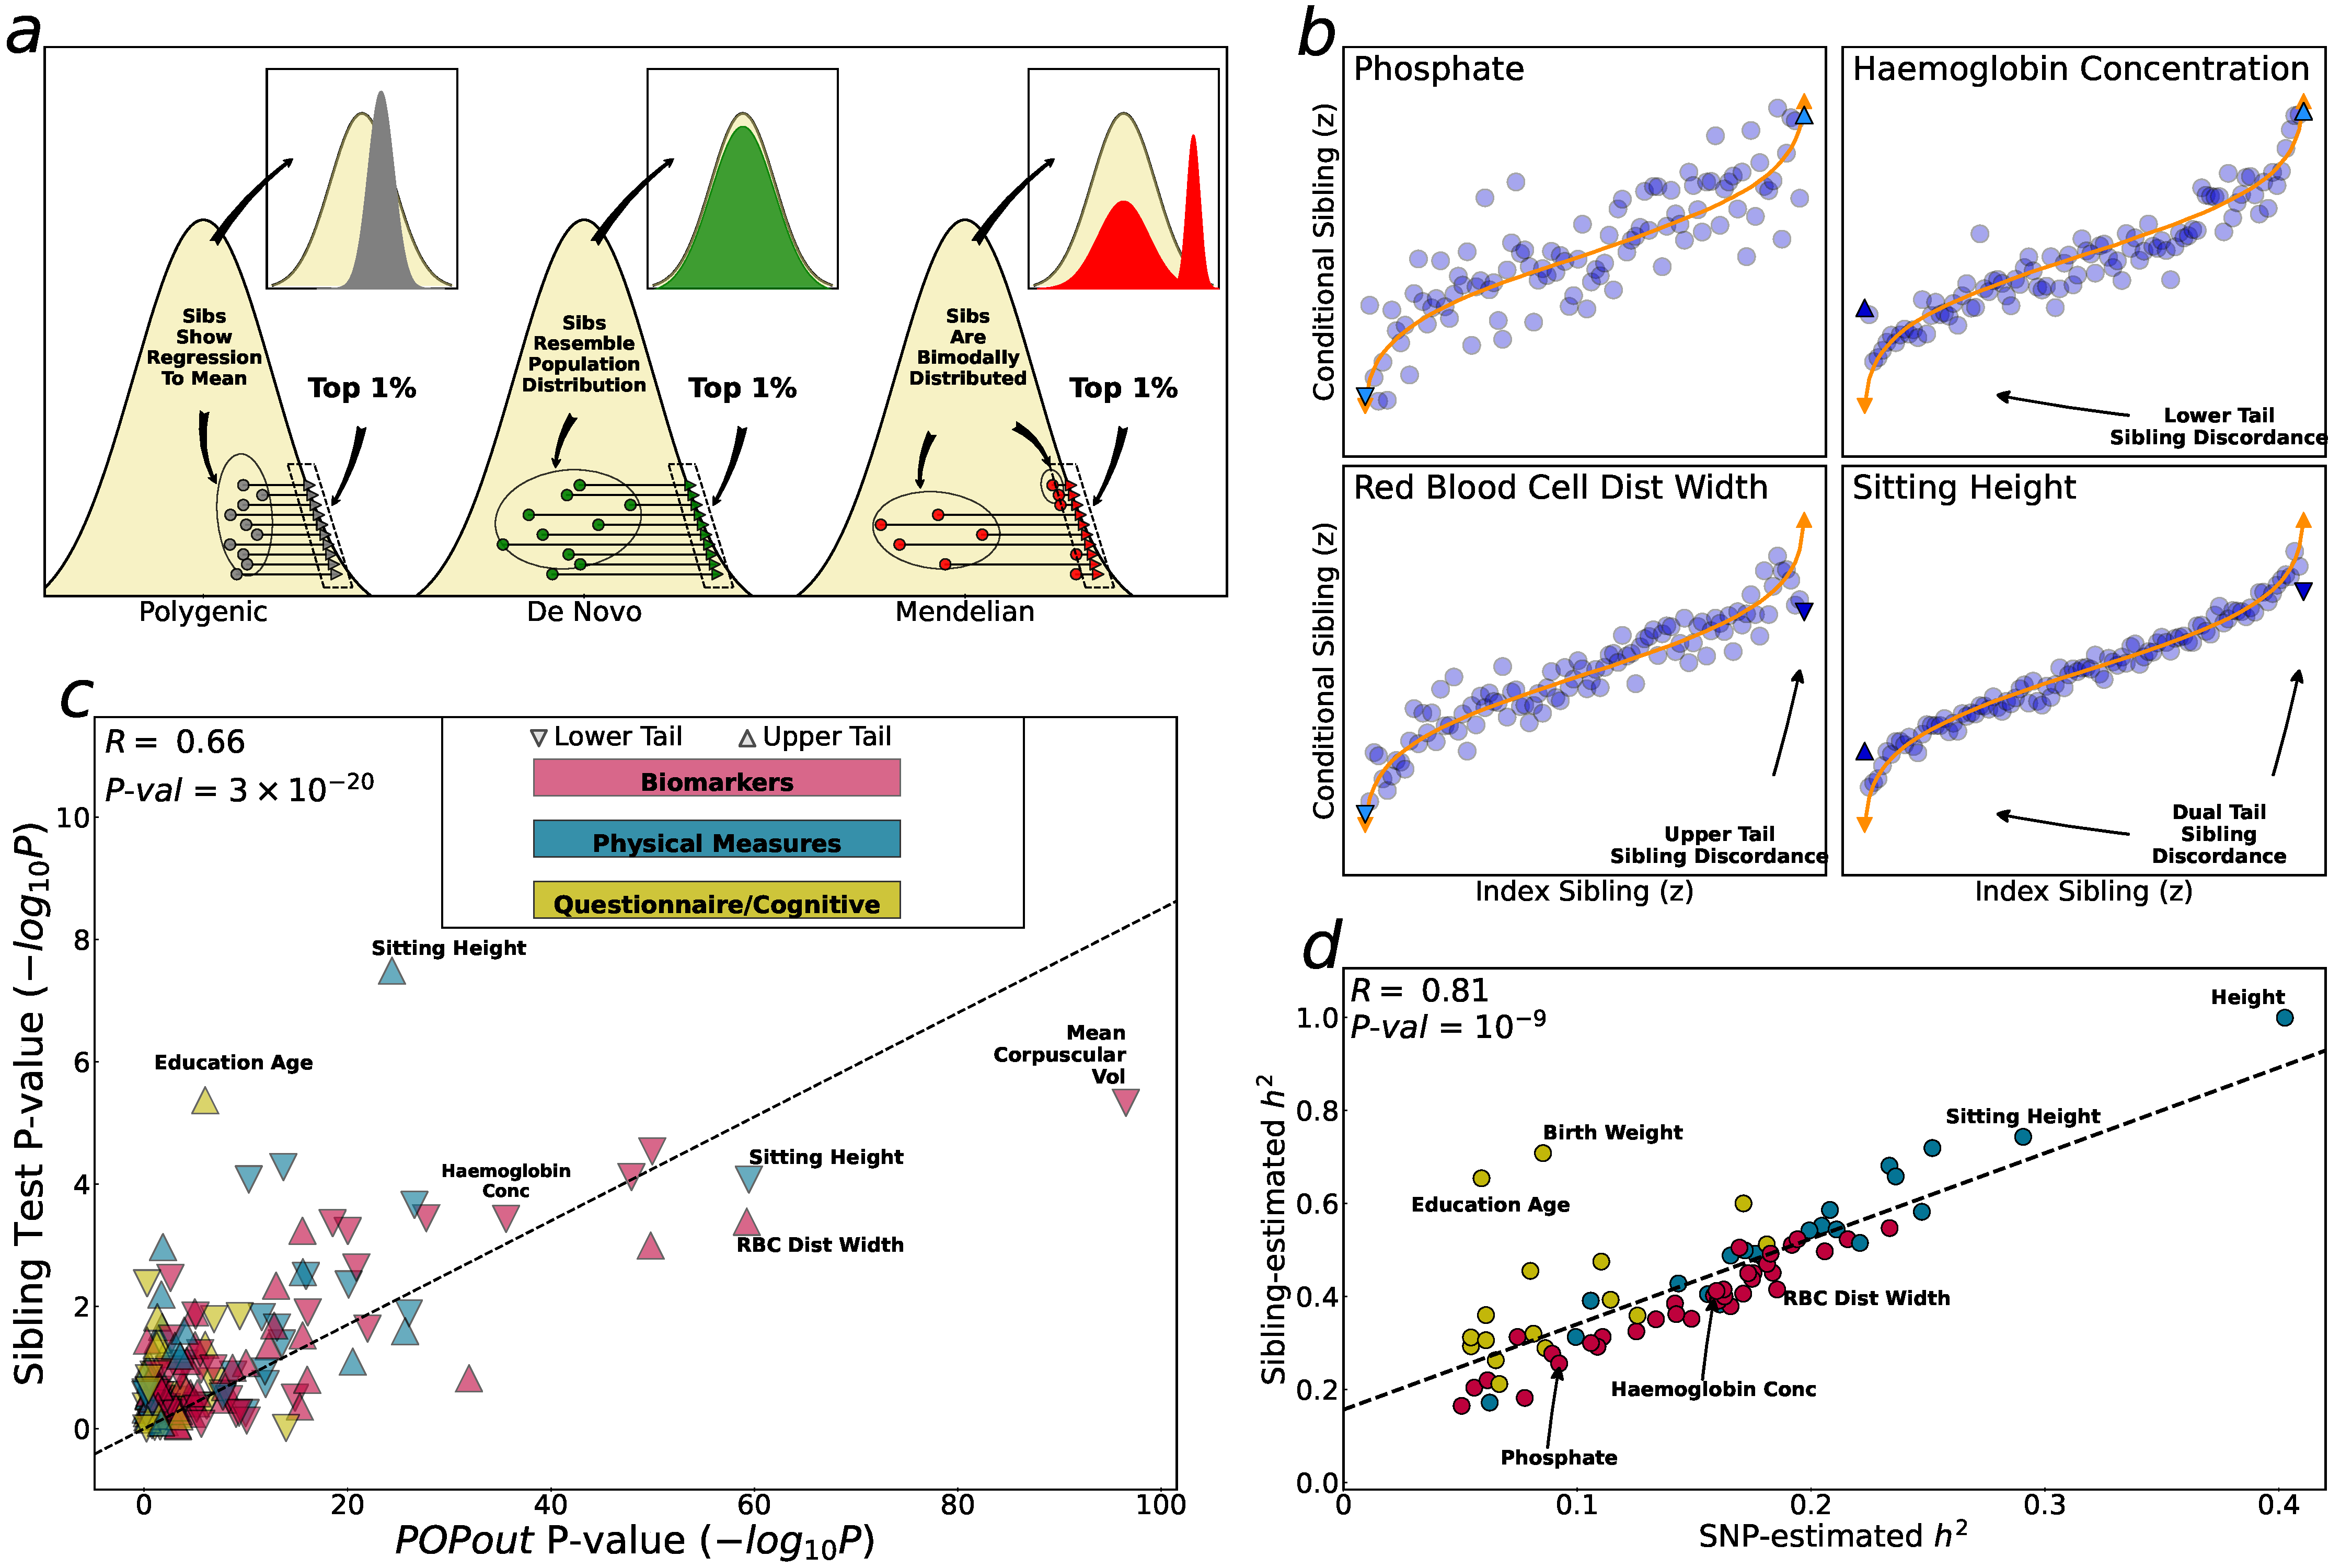
\includegraphics[trim=0cm 0cm 0cm 0cm, clip, width=\linewidth]{Figures/Fig3.pdf} \end{maybe} 
\caption{\footnotesize{{\bf Tail architecture inferred from siblings.}
    \textbf{(a)} Schematic of relationships between sibling trait
    values under polygenicity, de novo variants of large effect in one
    sibling and rare variants of large effect within families --
    Mendelian variants. \textbf{(b)} LDscore regression SNP
    heritability plotted against heritability estimated from sibling
    pair trait similarity using European UKB samples.  \textbf{(c)}
    Index sibling trait quantile (in 1\% increments) plotted agaisnt
    mean trait value of conditional sibling in quantile for the four
    traits selected with different POPout characteristics (Fig
    2a). \textbf{(d)} POPout P-values plotted against meta analysis
    P-values of sibling de novo and Mendelian tests on $-\log_{10}$
    scale for upper and lower tails of all 74 traits. Correlation and
    significance calculated using Pearson correlation.}}
\label{fig3} \end{figure} \FloatBarrier





The UK Biobank (UKB) includes 17,289 sibling pairs of European 
ancestry available for our STANDout analyses, none of which 
were included in our population-based analyses. There were too 
few sibling pairs of non-European ancestry for a sufficiently 
powered sibling analysis. Data across all 74 traits were 
available for analysis. Replicating our POPout analysis, our 
STANDout analysis showed no departure from polygenic expectations 
for phosphate, showed a significant lower tail STANDout effect 
for haemoglobin concentration (P=X), a significant upper tail 
STANDout effect for red blood cell distribution width (P=Y), 
and significant effects in both tails for sitting height 
(Fig.~\ref{fig:3b}; see Fig.~\ref{fig:2a} for comparison). 
More broadly, our sibling-based STANDout analyses replicated our 
population-based POPout analyses across the 74 traits extremely 
well (Fig.~\ref{fig:3c}; $R = 0.66$, $P = 3 \times 10^{-20}$). 
This is reassuring given that the two methods use such
orthogonal approaches and types of data. Further reassurance 
of the validity of our sibling-based method is provided by 
the strong correlation ($R = 0.81$, $P = 2 \times 10^{-9}$) 
between SNP-based heritability ($h^2$), estimated by the 
popular LD score regression approach~\cite{LD_score_regression}, 
and the sibling-based $h^2$ estimated as a key parameter in 
the STANDout approach (Fig.~\ref{fig:3d}).


\subsection*{Selection shapes tail architecture} 

In previous sections, we demonstrated that there are 
pervasive departures from our null model, which assumes 
polygenic architecture and jointly Gaussian environmental 
factors, in the tails of complex traits. However, these 
may still be due to unaccounted for non-Gaussian environmental 
risk factors. Here, we investigate evidence for our 
hypothesized cause of these tail departures from expectations; 
namely, that they are caused by the enrichment of rare, 
large-effect alleles in the tails due to selection on the 
trait constraining large-effect alleles to low frequency 
(Fig.~\ref{fig:1}). Backman et al.~\cite{Backman_2021} conducted 
the most comprehensive trait-wide analysis of UK Biobank 
exome sequence data to date, and here we utilize their 
results to investigate whether traits with significant tail 
departures are associated with a greater number of significant 
exome variants (or ‘hits’), with effects in the expected 
direction. Considering our four example traits, phosphate has
two exome hits with positive and four with negative 
effect sizes, haemoglobin concentration has eight with 
positive and twelve with negative effect sizes, red blood 
cell distribution width has twenty-eight with positive and 
five with negative effects, and sitting height has ten with 
positive and twenty with negative effects (Fig.~\ref{fig:4a}). 
Across the 74 traits, we find that $POPout$ effect sizes from 
our primary analysis are significantly positively 
correlated ($R=0.35$, $P=2\times10^{-5}$) with the 
number of exome hits with effects in the direction 
relating to the tail of the POPout 
effect (Fig.~\ref{fig:4b}). This provides direct 
support for the observed complex tail architecture 
being underlain by rare alleles. Findings by Fiziev and 
colleagues~\cite{Fiziev_2023} offer further support. 
The authors derived rare PRS across a range of quantitative 
traits in the UKB using their PrimateAI algorithm, and 
found that their rare PRS performed particularly well in 
predicting individuals with extreme trait values. 
However, we highlight one result that suggests that rare 
PRS may perform poorly for traits under extremely strong 
selection. The trait with the most significant $POPout$ 
effect in the questionnaire/cognitive category 
(Fig.~\ref{fig:2b}) was \textit{Age at Menopause}, 
which had an effect consistent with rare allele 
enrichment in the lower tail; yet the exome data showed 
no hits of negative effect (Fig.~\ref{fig:4c}). However, 
given the rationale for early age of menopause being 
under particularly strong negative selection, it may 
be that only ultra-rare alleles of large effect 
remain in the population, producing a PRS regression-to-the-mean 
in the tail but little signal in exome data.

%%%%%%%%%%%%%%%%%%%%%%%%%%%%%%%%%%%%%%%%%%%%%%%%%%%%%%%%%%%%%%%%%%%%%%%%
%%%%%%%%%%%%%%%%%%%%%%%%%%%%  FIGURE 4 %%%%%%%%%%%%%%%%%%%%%%%%%%%%%%%%%
%%%%%%%%%%%%%%%%%%%%%%%%%%%%%%%%%%%%%%%%%%%%%%%%%%%%%%%%%%%%%%%%%%%%%%%%
\FloatBarrier \begin{figure}[!h] 
\begin{maybe}{showFig} \includegraphics[trim=0cm 0cm 0cm 0cm, clip, width=\linewidth]{Figures/Fig4.pdf} \end{maybe} 
\caption{\footnotesize{{\bf Concordance between POPout effect size and
      rare variants of large effect and selective preasure.}}
  \textbf{(a)} Trumpet plots (minor allele frequency v effect size) of
  genome-wide significant variants for the four traits selected with
  different POPout characteristics (Fig 2a). \textbf{(b)} POPout
  effect size plotted against the number of genomewide significant
  variants with MAF<1\% for 58 traits with overlapping exome sequence
  results.  For upper tails positive variant effects are counted and
  for lower tails negative variant effects are counted.  Correlation
  and significance calculated using Pearson correlation. \textbf{(c)}
  Age of menopause: PRS quantile vs. trait mean and trumpet plot.
  \textbf{(d)} Residualised trait value plotted against relative
  lifetime reproductive success for 16 example traits.  Best model fit
  to the data, selected by BIC considering all models with and without
  linear and quadratic terms, are shown by dashed lines. Model
  selected by BIC used to classify selective pressure acting on the
  traits. \textbf{(e)} POPout effect size grouped by model selection
  category for \need{X traits}. Test for difference between upper and
  lower tail mean effect sizes calculated \need{by....}  \textbf{(f)}
  Spearman rank correlation between four proxy measures of fitness and
  POPout effect size. For each fitness measure, correlation was
  calculated between the mean of the fitness measure in individuals in
  the upper and lower 1\% trait tails and POPout effect size for the
  corresponding tail across 74 trait tails.}
\label{fig4} \end{figure} \FloatBarrier




To gain greater insight into how selection may impact variation 
in genetic architecture across the trait continuum, we 
performed simulations using the forward-in-time population 
genetic simulator SLiM~\cite{BC_2019}. Using standard population 
genetic parameter settings (see Methods), we simulated genetic 
variation data and a ‘trait’ calculated as the sum of 
genome-wide alleles, with effect sizes drawn from a Gamma 
distribution. After an initial burn-in period under neutrality, 
the trait was subject to stabilizing selection or strong 
stabilizing selection. After stabilizing selection, rare alleles 
were enriched in the trait tails compared to under neutrality, 
and this effect was more pronounced for ultra-rare alleles and 
after strong stabilizing selection (Fig.~\ref{fig:4d}). Under 
neutrality, approximately 1\% of simulated individuals in the 
top trait centiles harbored rare alleles of sufficiently large 
effect to cause their extreme trait value, whereas under strong
stabilizing selection, about 28\% of individuals in the tails 
carried such alleles. As a result, the trait tails showed a marked 
difference between trait value and PRS calculated from common alleles 
only across replicated (Fig.~\ref{fig:4e}). These simulations 
suggest that selection can have a critical impact on how genetic 
architecture varies across the trait continuum and could, thus, 
have played an important role in the observed departures from 
polygenic expectations in trait tails here.


To test this more explicitly in our real data, we apply a 
method~\cite{Sanjak_2018} for inferring ongoing selection from 
lifetime reproductive success to our 74 traits in the UKB 
data (see Methods). We use Bayesian Information Criteria (BIC) 
to distinguish 'no selection', 'positive', 'negative', and 
'stabilising' selection in the fitted models (Fig.~\ref{fig:4f}). 
Next, we stratify the POPout results of the primary analysis into 
traits according to the categories of inferred selection and test if 
the POPout effects reflect the inferred selection (Fig.~\ref{fig:4g}). 
Despite the snapshot into historical selection provided by 
contemporary reproductive success, POPout effects were reflective 
of inferred selection. There were no significant differences in POPout 
effect between lower and upper tails under no selection (P=X) and 
non-directional stabilising selection (P=Y), as expected, significantly 
larger POPout effects in the lower tail for traits with inferred 
positive selection (P=Z) and significantly larger POPout 
effects in the upper tail for traits under inferred negative 
selection (P=Q), as expected. Finally, we tested for associations 
between POPout effects and proxy measures of fitness.



%%%%%%%%%%%%%%%%%%%%%%%%%%%%%%%%%%%%%%%%%%%%%%%%%%%%%%%%%%%%%%%%%%%%%%%%%%%%%%%%%%%%
%%%%%%%%%%%%%%%%%%%%%%%%%%%%%%%%%%%%%%%%%%%   DISCUSSION - START  %%%%%%%%%%%%%%%%%%
%%%%%%%%%%%%%%%%%%%%%%%%%%%%%%%%%%%%%%%%%%%%%%%%%%%%%%%%%%%%%%%%%%%%%%%%%%%%%%%%%%%%
\clearpage \newpage
\section*{Discussion} \label{sec:discussion} 
Our POPout replication results suggest that the observed 
departures from polygenic expectations in the tails of many 
quantitative traits is a stable, replicable, global phenomena, 
supporting our hypothesis; namely, that selection has driven 
high-impact, rare alleles to the tails of many human traits, 
resulting in heterogenous architecture that deviates 
substantially from the infinitesimal model in the tails.

Limitations: 

Non-Eur considered as a single group. Combining individuals of high diversity 
into a single group prevents evaluation of potential heterogeneity, 
but relatively large sample sizes are required to make inference about 
distribution tails and such replication is conservative.

%%%%%%%%%%%%%%%%%%%%%%%%%%%%%%%%%%%%   END DISCUSSION %%%%%%%
%
%
%
%
%
%
%
%
%
%
%
%
%
%
%
%
%
%
%
%
%
%
%


%
%
%
%
%  PREV: INTRO, NEXT: RESULTS 
%
% 
% 
% 
% 
% 
% 
% 
% 
% 


%In \fref{fig:evo}{d-g} the results from our simulation are shown; stabilising 
%selection reduces the effect size of common variants (\fref{fig:evo}{d,e}) and enriches the tails 
%for rare variatns (\fref{fig:evo}{f}) leading to POPout regression in PRS models that omit rare variants (\fref{fig:evo}{g}). 


%%%%%%%%%%%%%%%%%%%%%%%%%%%%%%%%%%%%%%%%%%%%%%%%%%%%%%%%%%%%%%%%%%%%%%%%
%%%%%%%%%%%%%%%%%%%%%%%%%%%%  FIGURE 2 %%%%%%%%%%%%%%%%%%%%%%%%%%%%%%%%%
%%%%%%%%%%%%%%%%%%%%%%%%%%%%%%%%%%%%%%%%%%%%%%%%%%%%%%%%%%%%%%%%%%%%%%%%

%\clearpage \newpage 
%\section*{Results} \label{sec:results} 

%Motivated by \need{simulated results that demonstrating the relationship 
%between selection, rare variants and POPout (see \fref{fig:sim})},  we selected UKB biobank traits 
%for analyses from the following categories  
%The traits analyzed in the following section were selected 
%from the UK-Biobank categories 
%\textit{Biomarkers}, \textit{Physical Measures}, 
%\textit{Touchscreen Questionnaire} and  \textit{Cognitive Tests}.  
%Continuous traits from these categories were standardised by regressing 
%out the effects of age, sex, and known environmental and technical factors 
%and then applying an inverse-normal transformation (see \textit{Methods: Trait Normalisation}).  
%Samples were then split in half, GWAS was carried out using Plink \cite{bt_10}, 
%and heritability and pairwise genetic correlation was estimated using LDscore \cite{ldsc}.
%Applying quality controls for sample size, heritability, skew, and oligogenicity and 
%removing strongly correlated traits resulted in the set of 74 traits (see \textit{Methods: Trait QC}), 
%used for the POPout associated analyses conducted across the large number of European ancestry 
%samples in the UK Biobank and replicated three ways: 
%across a subset of repeated measures European ancestry samples in the UK Biobank, 
%acorss a subset of non-European ancestry samples in the UK Biobank, and, where applicable, 
%across European ancestry samples in the All Of Us Biobank (see \textit{Replication}). 


%\subsection*{The POPout Test} ~\\ 

%Conceptually, POPout occurs when when samples in the tails of the trait phenotype 
%distribution have polygenic scores that significantly depart from expectation.  
%To quantify this phenomenon we have developed the \textit{POPout test} which regresses
%PRS-On-Phenotype to estimate the effect size, direction, and significance of departure from expected PRS 
%for individuals in the lower and upper 1\% of the trait distribution (see \textit{Methods}).  

%Applying this test to the European ancestry samples in the UK-biobank reveals widespread departure 
%from expectation across the 74 traits analysed.  Correcting for multiple tests (5\% false discovery threshold), 
%68 of 74 traits have significant POPout effects in one or both tails and that the vast majority (90\%) of these 
%effects are positive - i.e. reflect regression to the mean or unexpectedly mild risk scores - 
%which is consistent with rare variants of large effects in individuals of the trait tails. 
%\dref{fig:pop}{a} illustrates the three broad types of tail effects by plotting trait quantile, 
%in 1\% increments, versus mean PRS in the quantile for four index traits: 
%\begin{itemize} 
%\item \textit{Phosphate} - Selected because it has no observable $POPout$ Effect in either tail.  
%\item \textit{Haemoglobin Concentration} - selected for most significant POPout regression in lower tail only, 
%\item \textit{Red Blood Cell Distribution Width} - selected for most significant POPout regression in upper tail only, 
%\item \textit{Sitting Height} - selected for most significant POPout regression in both tails (minimum value).   
%\end{itemize} 
        

%\noindent \dref{fig:pop}{b} enumerates the POPout tail effects for all traits analyzed, separated into three logical UKB categories, \textit{Biomarkers}, \textit{Physical Measures} 
%and \textit{Questionnaire/Cognitive}.  Again positive POPout effects (regression to the mean) predominate, especially with respect to larger effects: 22 tails have 
%positive POPout effects greater than 0.25 while none have negative POPout effects less than 0.25.  Here we also observe that POPout regression is 
%most common in \textit{Biomarkers} category (79\% of tails) and least common in \textit{Questionnaire/Cognitive} category (43\% of tails). Overall 
%we observe a moderate relationship ($R=0.23,Pv=0.018$) between POPout regression and trait heritability, suggesting that POPout regression is 
%not driven primarily by environmental effects.  

%\dref{fig:pop}{c} illustrates the impact that tail $POPout$ has on the reliability of PRS model to predict phenotype in the upper tails.  
%For both traits shown, \textit{Haemoglobin Concentration} and \textit{Red Blood Cell Distribution Width} the relative odds ratios are 
%equal to expectation when "case" is defined very liberally - as being in lower or upper 25\% of the distribution but underperform in 
%the presence of $POPout$ when "case" is defined conservatively - being in the lower or upper 1\% of the distribution.  
%With respect to \textit{Haemoglobin Concentration}, where lower tail $POPout$ is present, the relative odds ratio for the lowest $PRS$ 
%quantile ($5\%$) when case is defined as being in the lower 1\% is only 1.5, which is far below expectation and far below the 
%upper tail analogue (top quantile ($95\%$ predicts case defined by upper 1\%) which is 3.5. 
%With respect to \textit{Red Blood Cell Distribution Width}, where upper tail $POPout$ is present, the relative odds ratio for the largest $PRS$ 
%quantile ($95\%$) when case is defined as being in the upper 1\% is only 1.7, which is far below expectation and far below the 
%lower tail analogue (bottom quantile ($5\%$ predicts case defined by lower 1\%) which is 5.1. This shows that while the presence of 
%$POPout$ in one or both tails does not preclude overall predictive power as defined using $PRS$ $r^2$ it can cause the $PRS$ to obtain 
%all its predictive power by using the moderate range of the distribution, causing $PRS$ models to describe the genetic architecture that 
%underlies a range of moderate phenotypes that excludes the extremes where disease is more likely to manifest. 
%

%In figure \dref{fig:pop}{d} the results of three flavours of $POPout$ replication performed on $POPout$ effect sizes is shown. 
%In each replication dataset, matching traits with at least five thousand samples that passed our \textit{$POPout$ regression QC} 
%mentioned above were included and the Pearson correlation across the $POPout$ tail effect sizes was calculated. 



%Replication across the mean in a small samples of repeated measures (50 traits, $R=0.71,Pvalue=2.3 \times 10^{-16}$) 
%in UKB samples of European ancestry demonstrates that $POPout$ effects are unlikely to be caused by random measurement errors that drive individuals to the tails of the distribution. 
%Replication in UKB-samples of Non-European ancestry (54 traits, $R=0.63,Pvalue=3.7 \times 10^{-13}$) 
%demonstrate that $POPout$ is not an ancestry specific phenomenon. 
%Lastly, replication in the $All of Us$ cohort (28 traits, $R=0.59,Pvalue=1.6 \times 10^{-6}$) 
%demonstrate that $POPout$ is not a UKB specific phenomenon as a matched ancestry sample 
%in a different country also has similar results. For more information on replication please see \textit{supplement}. 
%Interestingly, the correlation across ancestry (UKB European and non-European) samples is higher than the 
%within ancestry across biobank correlation (UKB European and All of Us European) which suggests that despite 
%accurate PRS prediction not being portable across ancestry that POPout regression is still portable across ancestry groups. 









% trained comprised





%In \fref{fig:rep}{a} trait quantile is plotted in 1\% increments versus mean PRS in the quantile of our index traits, with 
%\textit{Height} and \textit{Weight} subsituting for \textit{Phosphate} and \textit{Sitting Height} which are 
%not available in the the \textit{All Of Us} dataset.  Visual concordance can be observed across the European ancestry 
%repeated measures, the non-European samples and the \textit{All Of Us} dataset.  In \fref{fig:rep}{b} POPout effect 
%sizes and confidence intervals are shown for all traits avaialble across the biobanks.  In \fref{fig:rep}{c-e} the 
%significant correlations across averaged measures, non-European samples, and \textit{All Of Us} are shown.  Interestingly, 
%the correlation across ancestry (UKB European and non-European) samples is higher than the correlation across biobanks 
%but within ancestry which suggests that despite accurate PRS prediction not being portable across ancestry that 
%POPout regression is still portable across ancestry groups. 








%%%%%%%%%%%%%%%%%%%%%%%%%%%%%%%%%%%%%%%%%%%%%%%%%%%%%%%%%%%%%%%%%%%%%%%%
%%%%%%%%%%%%%%%%%%%%%%%%%%%%  FIGURE 3 %%%%%%%%%%%%%%%%%%%%%%%%%%%%%%%%%
%%%%%%%%%%%%%%%%%%%%%%%%%%%%%%%%%%%%%%%%%%%%%%%%%%%%%%%%%%%%%%%%%%%%%%%%

%\clearpage \newpage
%\subsection*{\emph{Replication in Siblings}} ~\\
%Discordance between siblings in the tails of the trait distribution is
%indictive non-polygenic inheritance \cite{avi}. Furthermore, excess
%trait concordance between siblings can be indicative of shared
%Mendelian effects \cite{t_sibs}. \fref{fig:sib}{a} illustartes the
%expected impact of polygenicity, de novo, and Mendelian rare variants
%within sibling pairs. Expected sibling pair concordance under
%polygenicity can be used to test for (1) excess discordance between
%siblings in tails of trait distribution, indicative of de novo
%mutations of large in one sibling and (2) excess concordance between
%siblings in tails of trait distribution, indicative of shared
%Mendelian effects \cite{t_sibs}. These tests are derived from the
%conditional sibling distribution under polygenicity, this distribution
%also allows heritability to be estimated \cite{t_sibs}.

%Applying this model to the sibling data in the UKB to estimate $h^2$, 
%we find a correlation between snp h2 and sibling h2 in \fref{fig:sib}{b}.  
%As shown in \fref{fig:sib}{c}, we use this model to infer the presence of rare variant 
%architecture in our index traits and find lower tail discordance 
%in \emph{Haemoglobin Concentration}, upper tail discordance in 
%\emph{Red Blood Cell Distribution Width} and dual ail discordance 
%in \emph{Sitting Height}, all of which match the result of the POPout analyses. 
%We also find an overall significant relationship between sibling test pvalue and the POPout pvalue across all 74 traits \fref{fig:sib}{d}. 
%Interestingly, this relationship varies across category, pearson correlation is $0.80$ across the \textit{Biomarker} group, 
%$0.60$ across the \textit{Physical Measures} and insignificant the lower heritability \textit{Questionnaire/Cognitive} category suggesting again 
%that concordance between POPout effects and sibling discordance is not the result environmental causes alone. 










%\clearpage \newpage



%\noindent The genetic mechanism proposed to explain $POPout$ involves the confluence 
%of genetic selection away from one or both tails, an enrichment of rare variants in those tails, 
%and PRS methods that typically restrict to common variants (MAF $>1\%$) that suffers in such tails.  
%Indeed, the exclusion of rare variants from PRS has already been shown to 
%reduce PRS performance \citep{rares1}. \fref{fig:evo}{a} shows
%the relationship between MAF and effect sizes from significant
%associations derived from GWAS \citep{neale} and exome analyses
%\citep{backman} of UKB for our four index traits. For \textit{Haemoglobin
%Concentration} which exhibits lower tail regression we see a greater
%number of rare variants in the lower tail and for \textit{Red Blood Cell
%Distribution Width} which exhibits upper tail regression we see a
%greater number of rare variants in the upper tail. Sitting height,
%which exhibits dual tail regression, has a number of rare variants in
%both tails, however, there are more rare variants in the lower tail
%where the POPout effect is greatest. For \textit{Phosphate} which does
%not exhibit POPout in either tail there are much fewer rare
%variants of large effect.  These results are consistent with the hypothesis that
%rare variants of large effect that not accounted for in the
%common-variant PRS are responsible for tail POPout effects. 

%Indeed this relationship holds up across all traits analysed.  In 
%In \fref{fig:evo}{b} we observe a small but significant relationship
%between the magnitude of \textit{POPOut} regression in the tail and the number of rare
%variants in the tail across all trait tails analysed. However, we note that 
%while statistically significant, there are multiple traits with significant 
%\textit{POPout} scores for which almost no rare variants of substantially large effect 
%have been identified (see \fref{fig:evo}{c}).  This suggests that strong selection 
%may result in private variants that cannot be identified using population based sequencing.















%\subsection*{The Impact of Selection} ~\\
%Using adjusted lifetime reproductive success \citep{v_select, v_select2} as a proxy for selection 
%we classified the selective pressure acting on each trait (see \textit{Methods} - LRS) by fitting it an 
%optimal two parameter model ($Y_{LRS} = x_o+ \beta x + \gamma X^2$) as determined by BIC.  Shown 
%in \fref{fig:evo}{a}, most traits (65 of 74\%) have some relationship (ie. $\beta \neq 0$ or $\gamma \neq 0$) 
%between between adjusted lifetime success and trait quantile and the majority of them (43 of 65) 
%two thirds of traits (43 of 65) were classified as being under some form of stabilising ($\gamma < 0$) selection, which is 
%characterized by lower fecundity in the both tails of the trait distribution.  
%This may be the result of general fitness  favoring the trait mean or the result of sex specific selection 
%that averages to produce this relationship \citep{v_select}.  Only two traits were classified as under disruptive 
%selection ($\gamma > 0$) which is characterised by greater fecundity in both trait tails. 

%Irrespective of their gamma parameter, 57 trait models included a nonzero directional beta parameter.  
%In \fref{fig:evo}{b} we see that traits under positive selection have significantly more POPout regression 
%in the lower tail and that traits under negative selection have signficicantly more POPout regression 
%in the positive tail - which is in line with theoretical and simulated predictions that suggest that 
%negative selection drives an enrichment of rare variants in the tail which reducing polygenicity and 
%driveout POPout regression.  



%\subsubsection*{Tail Fitness} ~\\ 

%In addition to model selection on adjusted lifetime reproductive sucess we analysed the 
%relationship between five ranked fitness related measures associated with \emph{de novo} etiology 
%and ranked POPout regression across all 148 tails analysed.  Shown in \fref{fig:evo}{c}, we find that 
%while POPout regression is associated with less less offspring in both sexes, that this effect may 
%be stronger in males.  Additionally we find that while neither the number of illnesses or miscarriages and 
%stillbirths are significantly associated with POPout regression that paternal age \cite{pat} 
%further suggesting that private variants may be driving some of the POPout signal. 

%%%%%%%%%%%%%%%%%%%%%%%%%%%%%%%%%%%%%%%%%%%%%%%%%%%%%%%%%%%%%%%%%%%%%%%%%%%%%%%%%%%%
%%%%%%%%%%%%%%%%%%%%%%%%%%%%%%%%%%%%   END RESULTS %%%%%%%%%%%%%%%%%%%%%%%%%%%%%%%%%
%%%%%%%%%%%%%%%%%%%%%%%%%%%%%%%%%%%%%%%%%%%%%%%%%%%%%%%%%%%%%%%%%%%%%%%%%%%%%%%%%%%%
%
%
%
%
%
%
%
%
%
%
%
%
%
%
%
%
%
%
%
%
%
%
%
%
%
%
%
%
%
%
%
%
%
%
%
%
%
%
%
%
%
%
%
%
%
%
%
%
%
%
%
%
%
%
%
%
%
%
%%%%%%%%%%%%%%%%%%%%%%%%%%%%%%%%%%%%%%%%%%%%%%%%%%%%%%%%%%%%%%%%%%%%%%%%%%%%%%%%%%%%%%   
%%%%%%%%%%%%%%%%%%%%%%%%%%%%%%%%%%%%%%%%%%%   METHODS - START     %%%%%%%%%%%%%%%%%%%%
%%%%%%%%%%%%%%%%%%%%%%%%%%%%%%%%%%%%%%%%%%%%%%%%%%%%%%%%%%%%%%%%%%%%%%%%%%%%%%%%%%%%%%
\clearpage \newpage 
\section*{Methods} 
\vspace*{0.2cm} 
%%%%%%%%%%%%%%   METHODS 1- DATA PROCESSING %%%%%%%%%%%%
\subsection*{Data Processing} ~\\
\vspace*{-0.5cm} 
\subsubsection*{UK Biobank Genetic Data} ~\\
The UK Biobank (UKB) is a prospective cohort study of approximately
500,000 participants recruited across the United Kingdom from 2006 to
2010 \citep{ukb}. Phenotype data of anthropometric, biological and
lifestyle measures were collected at baseline and in follow-up surveys, with
further linkage to health and disease record data. The genetic dataset
consists of 488,377 samples genotyped at 805,426 SNPs.
To define population ancestries, 4-means clustering analysis was
conducted on the first two principal components (PCs) of the genotype
data. Samples were then projected onto 1000 Genomes PCs to infer
ancestry, resulting in 461,931 European, 11,074 South Asian, 7,935
African, 2,585 West Asian, 2,550 East Asian, 1,619 and admixed
samples.

Subsequent to clustering, standard quality control (QC) procedures
were applied independently to each ancestry cluster. SNPs with a minor
allele frequency (MAF) $<$ 0.01, genotype missingness > 0.02, or
Hardy-Weinberg equilibrium test $P$-value $< 10^{-8}$ were
excluded. Samples exhibiting high levels of missingness or
heterozygosity, inconsistencies in genetic-inferred and self-reported
sex, or displaying aneuploidy of the sex chromosomes, were removed in
accordance with recommendations from the UKB data processing team
\citep{ukb_qc}.  For the analyses in the general population, a greedy
algorithm was employed to remove related individuals that maximises
sample retention while removing all third-degree relatives (kinship
coefficient > 0.044) \citep{erase}.  After these QC steps, 411,949 unrelated    % THESE NUMBERS DON'T ADD UP 
individuals remained, of which 387,235 were of European ancestry. Included 
among the European ancestry cluster were 18,340 individuals with repeated 
measures that were set aside, along with the 24,476 non-European individuals, 
for replication analyses (see below). This resulted in up to 369,133 unrelated 
European ancestry individuals for the primary $POPout$ analyses (see below). 

For the sibling analyses (see below), sibling pairs were selected by first
identifying first-degree relatives, defined as those with kinship
coefficient within the range 0.177 and 0.354 (expected value for
siblings is 0.25) to account for the expected variation among siblings \citep{sib1}. 
Only individuals of European ancestry were included in the sibling analyses due to 
insufficient statistical power of the non-European ancestry samples \citep{t_sibs}. 
The proportion of SNPs with zero identity-by-state (IBS0) was used to distinguish 
sibling pairs from parent-offspring pairs, since parent–offspring pairs have
IBS0$\approx$0 across the autosomes. It has been shown in the UKB that
there is good separation between pairs of first degree relatives at
IBS0=0.00112 \citep{sib1} and, thus, sibling pairs were selected as
those exceeding this threshold. This provided a total of 17,289 sibling pairs 
for analysis.

\subsubsection*{Quantitative Trait QC} ~\\
\vspace*{-0.6cm} 
\paragraph*{Trait Selection} ~\\ 
We considered all traits from the categories \textit{Biomarkers} (453 traits), \textit{Physical Measures} (271 traits), the \textit{Touchscreen Questionnaire} (396 traits) and \textit{Cognitive Function} (134 traits) 
to provide a broad group of well-studied, heritable traits. To minimise non-genetic causes of trait values, we then removed all individuals with a cancer diagnosis (34,698), on insulin treatment (1,311) or who were pregnant at baseline (109). We also removed 64,043 individuals on statins and other cholesterol-lowering drugs from the \textit{Blood count} and \textit{Blood Biochemistry} subcategories and 29,395 individuals
on heart rate medication from the \textit{Arterial stiffness} and \textit{Blood pressure} subcategories.
Next, to ensure that extreme outliers do not impact results, we removed all samples that had trait values six standard deviations or more from the mean. After these removals, we defined quantitative traits as 
those containing at least 10 distinct values and whose top two modal values comprise less than 
half the samples. Finally, we removed all traits with < $100,000$ samples remaining in our 
primary dataset of unrelated European ancestry individuals, resulting in a set of 180 quantitative 
traits. These traits were then residualised as described below. 

\paragraph*{Trait Residualisation} ~\\
To minimise the impact of environmental risk factors, trait values were 
residuallised within each ancestry group (European and Non-European) by applying a linear regression 
model to each trait, with covariates for $age$, $age^2$, $age^3$, sex, menopause status, %(Field ID: 2724), 
type-II diabetes status, coronary artery disease status, alcohol intake (Field ID: 1558), 
smoking (categorical - Field ID: 20116 and continuous - Field ID: 1239), 
batch, centre, and the first 40 genetic PCs.  
At this stage, traits residuals with an absolute skew $>2$ \cite{skew_book} 
in the larger European ancestry group were removed to avoid measurement bias and 
the remaining trait values were standardised using a rank inverse 
normal transform on the residuals. This provided traits adjusted for by key environmental factors, genetic 
PCs, and with relatively low skew, transformed to have standard normal distributions for all analyses. 

\paragraph*{Further Trait QC} ~\\
To conduct our initial primary analyses, European ancestry UKB samples were split 
randomly into 50\% base and 50\% target data sets, for computing GWAS results and PRS (or "polygenic scores"), respectively. Then, for each trait, a GWAS was performed using the standardised trait values in the base data, applying PLINK-1.9 \citep{plink, bt_10}, while heritability and pairwise genetic correlations were estimated using LD score regression \cite{ldsc}.  To ensure that our PRS analyses are well-powered, we removed traits with heritability $h^2<5\%$ \cite{guide_paper}, while to ensure that the traits were essentially polygenic, rather than oligogenic, traits were removed for which a single SNP (MAF > 1\%) explained more than 2\% of trait variance \cite{2prule}. After these QC steps, 120 quantitative traits remained across all four categories. 

To verify that the traits were meaningfully different from each other, we considered their  
pairwise genetic correlations. More than half (64 of the 120) of the traits had pairwise genetic correlation $r_g>95\%$ with at least one other trait. Of these 64 traits, 22 had a single pairwise correlation above this threshold. For these 11 pairs of traits, the trait with higher heritability was selected for analysis.  The remaining 42 genetically non-unique traits came from two categories: \textit{ Bone-densitometry of heel}  and \textit{ Body composition by impedance}. Applying the same data maximisation algorithm used to select the maximum number of unrelated individuals \citep{erase}, we selected a further 7 traits (two bone-densitometry related and five body composition related) with pairwise $r_g<95\%$.  In addition to the 56 traits without high genetic pairwise correlations, and the 11 traits selected from correlated pairs, this resulted in a set of 74 traits for use in the primary analyses. % GIVE SOME ON AVERAGE NUMBERS OR BELOW - primary european and non, etc.  


\paragraph*{Initial PRS Analyses} ~\\
The 74 traits remaining after QC included 37 in the \textit{Biomarkers} category, 21 traits in \textit{Physical Measures} category, and 16 that were in either the \textit{Touchscreen Questionnaire} or \textit{Cognitive Function} categories.  In the primary unrelated European dataset, these traits had between of 50,109 and 167,857 (average 123,482) samples in each of the base and target datasets. For each (residualised) trait, PRSice \cite{prsice} was used to establish an optimal $P$-value threshold for computing PRS in the target data (2nd half of the data) using the \textit{FastScore} option (10 thresholds tested). Each PRS and corresponding trait were then used in the $POPout$ analyses, described below. While each PRS will be slightly overfit to the data due to training and testing within the same data, the use of only 10 $P$-value thresholds should minimise this overfitting, and overfitting of PRS to the trait should be independent, and in fact conservative, in relation to the results of the "POPout" analyses. This procedure optimised the sample size of the test data. None of the replication analyses (below) were subject to any overfitting since they all corresponded to out-of-sample data. 

%\vspace*{0.4cm} 
\subsubsection*{Replication Dataset QC}
\paragraph*{European Ancestry Repeated Measures} ~\\
After initial QC (above), there were 18,340 European ancestry individuals 
with measurements repeated at a follow-up data collection five years after baseline. 
For these individuals, both measurements were normalised alongside 
the other European ancestry UKB samples, as described above, but held out of the base dataset. Then 
the residualised trait values from their two visits were averaged (mean) to provide a 
target subset of individuals for which random measurement error, or transient effects e.g. infections, are less likely to produce trait values in the tail. Across the 74 traits, there were between 
2,461 and 15,475 (mean: 10,699) unrelated individuals for repeated measure replication. \textcolor{red}{all 74 traits???}. PRS were calculated in this sample using the $P$-value threshold (and, thus, same SNPs) optimised for the relevant trait in the primary analyses, as well as the (same) effect size weights of the base GWAS. 

\paragraph*{Non-European Ancestry Individuals} ~\\
After initial QC (above), there were 24,476 non-European ancestry individuals. The trait values of 
these individuals were normalised alongside the European UKB individuals, as above, and PRS 
were calculated for the 74 traits of our primary analyses using \cite{prsice}. \textcolor{red}{all 74 traits???}.
PRS were calculated in this sample using the $P$-value threshold (and, thus, same SNPs) optimised for the relevant trait in the primary analyses, as well as the (same) effect size weights of the base GWAS. There were between 569 and 22,513 (average: 14,871) unrelated individuals for this cross-ancestry replication. 

\paragraph*{All of Us Cohort} ~\\
\emph{All Of Us} is a multi-ancestry biobank from the United States, utilising 
electronic health record (EHR) data in a cohort of individuals with a wider age 
range than the UKB ($\mu,\sigma$= 55.8,17.1 vs 56.5,8.1). 
Traits matching those analysed in our primary UKB analysis 
were identified through an initial database search and were 
then interrogated manually to determine if trait descriptions 
were sufficiently similar (see \textit{Supplemental Table}).  
All of Us provides ancestry categories, corresponding to definitions 
used within gnomAD \cite{gnomad}, 
the Human Genome Diversity Project \cite{hgdp}, 
and 1000 Genomes project \cite{tgp}.  
133,581  European ancestry individuals were extracted for analysis. %Too few individuals of non-European ancestry were avaialble for sufficient replication power.

Trait QC in All Of Us was conducted to match that performed in the UKB as closely as possible, given 
available trait information. First of all, individuals on statins were removed 
from the \textit{Blood count} and \textit{Blood Biochemistry} subcategories, and then the median measurement value for every trait (EHR data includes multiple measures) was selected and 
the age corresponding to that measurement was extracted. For each trait, outliers greater 
than six standard deviations from the mean were removed and a linear regression model was 
applied with covariates for $age$, $age^2$, $age^3$, sex, and the first 40 genetic PCs. A rank inverse normal transformation was applied to the regression residuals to provide standardised trait values, as for the UKB.

Genetic QC in All Of Us was conducted using standard filters, as used in the UKB.  SNPs with MAF $<$ 0.01, genotype missingness > 0.02, or Hardy-Weinberg equilibrium test 
$P < 10^{-8}$ were excluded. Samples exhibiting high levels of missingness or heterozygosity, 
inconsistencies in genetic-inferred and self-reported sex, or displaying aneuploidy of the sex 
chromosomes were removed and the same greedy algorithm used to maximise sample 
retention of unrelated individuals as used in the UKB, was applied here. Using the higher-powered 
publicly available European ancestry GWAS summary statistics generated from the entire UKB \cite{neale} to provide SNP weights, trait PRS were calculated \cite{prsice} using the same $P$-value threshold relevant to each trait and trained in the UKB European ancestry analysis (see above). 



%%%%%%%%%%%%%%   METHODS 2- DATA ANALYSIS %%%%%%%%%%%%

\vspace*{0.3cm} 
\subsection*{Data Analysis} ~\\
\vspace*{-0.4cm} 
\subsubsection*{POPout Analyses}

\paragraph*{The POPout Test}~\\ 
Here we describe the "PRS-On-Phenotype outlier", or \emph{POPout}, test, which is 
designed to identify departures from polygenic expectations in the tails of 
quantitative traits from population genotype data. In our application, we seek to identify 
departures due to genetic factors, and, thus, we first perform a regression of traits on 
environmental risk factors (as described above) and use the residuals as input to the test. The POPout test first applies a regression of PRS on trait values, in which both the PRS and trait are standardised to have a standard deviation of 1. The assumption of the test is that, under uniform polygenicity, there is a linear relationship in prediction of PRS from trait values, but that under reduced polygenicity in the tails the fitted regression values systematically overestimate absolute PRS values in the lower and upper quantiles (i.e. observed PRS for extreme trait values will be closer to the population mean PRS than according to linear regression). The residuals from the regression are considered according to quantiles of the trait, and two-tailed t-tests are applied to test whether the residuals are significantly different from zero. Here we applied the test to individuals in the bottom and top 1\% of the trait distribution to test for departures from polygenicity in the tails. The effect size in each tail is defined such that a positive effect is indicative of regression-to-the-mean in both the lower and upper tails, as follows:
\[
POPout \;effect = \frac{1}{n}\sum_i^n |{f(y_i)}| - |{PRS_i}|
\]
where, within the tested quantile, $f(y)$ is the predicted PRS from the regression given trait
value $y$ and $n$ is the number of observations.

\paragraph*{POPout regression QC} ~\\
An additional trait QC was applied to ensure the robustness of the
$POPout$ to its assumptions by ensuring that the $POPout$ test 
did not produce significant results in the middle of the trait distribution. 
Specifically, for each trait, two-sided t-tests for zero mean were
applied to the residuals assigned in each of the middle 80 centiles of
the trait distribution. Traits were deemed to fail QC if the smallest
$P$-value was significant at a Bonferroni-corrected level of 0.05 ($P$
$\le$ 0.05/80). Such traits were removed from our analysis.

\paragraph*{Evaluating Impact of POPout Effects on PRS Prediction} ~\\ 
To evaluate how observed POPout effects impact on the performance of 
polygenic score, or PRS, prediction, we emulate a scenario in which the 
quantitative trait underlies a binary outcome (e.g. as is the case for BMI 
underlying clinical obesity). We consider individuals above a specified 
trait threshold value to be cases and individuals below the threshold to 
be controls. We investigate thresholds at the 75\% and the 99\% points of 
the trait distribution. For each, we use the PRS to predict case/control 
status, and then generate a quantile plot, in which the odds ratio of the 
given quantile is estimated in relation to the central quantile via logistic 
regression (Fig.2c). Additionally, for each trait with $PRS$ $r^2$, we simulated 
a quantitative phenotype with trait values given by $T=r{PRS}+E$, where 
$PRS$ has a standard normal distribution and $E$ represents all other contributions 
to trait variance and is drawn from a normal distribution with mean 0 and 
variance $(1-r^2)$. This produces a simulated trait with a $\mathcal{N}(0,1)$ 
distribution and $PRS$ $r^2$. Using the same number of target samples 
used in the real data analysis for each trait, this simulation allows us to 
estimate the expected predictive performance of the PRS based on the 
corresponding $r^2$ and assuming uniform polygenicity throughout the 
trait distribution. \textcolor{red}{Should be able to do this analytically instead? 
Using Pearson-Aitken I think}

\vspace{0.4cm} 
\paragraph*{Replication of POPout Results}~\\ 
\vspace{-0.5cm} 
\paragraph*{Bootstrap Study To Establish Power of Replication Analyses} ~\\
In our primary analysis QC, we set a minimum sample size threshold of 100k in total 
(i.e. at least 50k target) samples. To explore whether our $POPout$ results are expected 
to replicate with smaller sample sizes, we repeatedly sampled subsets of between 1k and 50k target samples and performed the $POPout$ test in these subset or "bootstrap" samples. 
For each target sample of between 1k and 50k (incrementing by 5k), we performed 100 bootstraps 
across each of the 148 trait tails and counted the number that replicated at FDR 5\%.
\textcolor{red}{Is this true?}. We also calculated the correlation between the bootsrap 
POPout effects and those of the full data at each bootstrap sample size. As a result of 
this investigation, we imposed a minimum replication target sample size of 5000 to 
provide sufficient power for replication (see \textit{Supplementary Figure 1}). 


\paragraph{Replication Across Datasets} ~\\
We replicated our primary $POPout$ analyses in three different independent cohorts:  
\textbf{(1)} UKB European ancestry individuals with repeat measures (baseline and follow-up at $\sim$5 years), \textbf{(2)} Non-European UKB individuals, \textbf{(3)} the European ancestry samples in the US-based \emph{All Of Us} biobank. For each cohort, traits with at least 5000 samples, passing our standard QC (see above), were included.


%%%%%%%%%%%%%%%%%%%%%%%%%%%%%%%%%%%%%%%%%%%%%%%%%%%%%%%%%%%%%%%%%%%%%%%%
%%%%%%%%%%%%%%%%%%%%%%%%%%%%  FIGURE 3 %%%%%%%%%%%%%%%%%%%%%%%%%%%%%%%%%
%%%%%%%%%%%%%%%%%%%%%%%%%%%%%%%%%%%%%%%%%%%%%%%%%%%%%%%%%%%%%%%%%%%%%%%%

\subsubsection*{Sibling-based Test for Departures from Polygenic Architecture}~\\
We have already developed sibling-based tests of departures from polygenic expectations in trait tails caused by \emph{de novo} high-impact alleles or caused by rare alleles of large effect segregating in families ("Mendelian" effects) \cite{t_sibs}. Here we summarise the theoretical framework underlying those tests, and then describe the novel test used here that combines the two tests into a single omnibus test to identify general departures from population expectations due to either cause. \\
The conditional distribution of an individual's trait value given their sibling's trait value, assuming the infinitesimal model for genetic effects ("polygenicity") and normally distributed environmental factors, can be derived analytically \cite{t_sibs} as:

\begin{equation} p(s_2 \mid s_1 ) \sim \N\left(\frac{1}{2}s_1h^2,
1-\frac{h^4}{4}\right) \label{math:S2givenS1}
\end{equation}
where $s_1$ and $s_2$ denote the index and conditional-sibling trait
values, respectively, and $h^2$ is the trait heritability. Rare
large-effect alleles can produce deviations from this distribution,
particularly when concentrated in specific parts of the distribution, 
which may occur in the trait tails if these effects are very large 
and abundant. Specifically, rare large-effect alleles segregating 
in families - {\em Mendelian effects} - will result in excess trait 
similarity (or concordance) between siblings on average compared
to polygenicity. Conversely, a high-impact {\em de novo} mutation in one
sibling will result in excess dissimilarity (discordance) between siblings.

Our sibling-based test for enrichment of {\em Mendelian} effects \cite{t_sibs} evaluates 
the proportion of sibling pairs in which both siblings reside in a defined quantile of the trait distribution, which can be formulated as a score test with the following z-statistic:
\begin{align*}
z&=\frac{r-n\pi_0}{\sqrt{n\pi_0(1-\pi_0)}}
\intertext{where $n$ is the number of index siblings in the quantile $q$ 
under test, $r$ is the number of siblings pairs where both siblings have trait values 
in $q$ and $\pi_0$ is the expected proportion of sibling pairs in the quantile under polygenicity, which is given by:}
\pi_0&=\frac{1}{n}\sum_{i\in A_q} \left( 1 - \Phi \left(
\frac{\Phi^{-1}(q)  - \frac{s_1^{(i)}
h^2}{2}}{\sqrt{1-\frac{h^4}{4}}} \right)\right)
\end{align*}
where $n$ is the number of sibling pairs, $A_q$ is the set of 
index siblings in trait quantile $q$, $\Phi$ is the normal 
cumulative density function and $\Phi^{-1}$ is its inverse.

Our sibling-based test for enrichment of {\em de novo} effects constructs a z-statistic for the distance between index siblings in the tail of the trait
distribution and their conditional siblings, as follows:
\begin{align*}
  z&=\frac{\sum_{i\in A_q}s_2^{(i)}-\frac{1}{2}s_1^{(i)}h^2} {\sqrt{n(1-\frac{h^4}{4})}}
\end{align*}
For index siblings in the lower and upper tails, the alternative
hypotheses of $H_1: z>0$ and $H_1: z<0$ are tested as one-tailed t-tests, respectively. For further details, see Souaiaia et al \citep{t_sibs}.

The trait heritability, $h^2$, a required parameter in the {\em Mendelian} and {\em de novo} tests, is estimated from the sibling pairs by calculating the maximum likelihood of $h^2$ 
under the null hypothesis of the infinitesimal model (see above): 
\begin{equation*} \log \mathcal{L} \propto -n\log\left(1 -
    \frac{h^4}{4}\right) - \frac{1}{1-\frac{h^4}{4}} \sum_{i=1}^n
  \left( s_{2}^{(i)} - \frac{s_1^{(i)} h^2}{2}
  \right)^2
\end{equation*}

\noindent In order to test for general departures from polygenic architecture in the tails of 
quantitative traits, caused either by high-impact alleles that are either \emph{de novo} or 
that are segregating in families (i.e. rare alleles), we combine the results of the two tests 
using Fisher's method to give a $\chi^2$ statistic with 4 degrees of freedom: 

\begin{align*}
    \chi^2_4 = -2(\log(p_{Mendelian}) + \log(p_{de novo}))
\end{align*}

%%%%%%%%%%%%%%%%%%%%%%%%%%%%%%%%%%%%%%%%%%%%%%%%%%%%%%%%%%%%%%%%%%%%%%%%
%%%%%%%%%%%%%%%%%%%%%%%%%%%%  FIGURE 4 %%%%%%%%%%%%%%%%%%%%%%%%%%%%%%%%%
%%%%%%%%%%%%%%%%%%%%%%%%%%%%%%%%%%%%%%%%%%%%%%%%%%%%%%%%%%%%%%%%%%%%%%%%

\clearpage \newpage

\subsubsection*{Rare Variant and Selection Analyses} 

\paragraph*{Associations between POPout effects and Rare Variants} ~\\
Backman et al \cite{backman} provides results from exome sequencing analysis 
performed in the UK Biobank full exome data across 3994 traits, including 65 of 
the 74 traits analysed in our target set. For each of these 65 traits, in each tail, 
the number of genes with at least one significant (P$\le 2.18\times 10^{-11}$; significance 
threshold used in \cite{backman}) variant (deleterious, missense, predicted loss of function) or a genome-wide significant burden association is counted. Across the 130 trait tails, we calculate the Pearson correlation between the number of exome variants and the $POPout$ 
effect size (Fig.4b). 

\paragraph*{Relative Lifetime Reproductive Success} ~\\
The number of offspring is recorded in the UKB for both females and
males. Following the approach of Beauchamp \citep{v_select2}, samples were 
stratified into four birth cohorts (1934-42, 1943-48, 1949-55, 1956-65). Individual relative
lifetime reproductive success, $Y_{rLRS}$, was then calculated by
dividing the number of offspring of each individual by the cohort
mean. Following Sanjak et al \citep{v_select}, the presence and
direction of selective pressure acting on traits was inferred by
fitting the following regression model:
\begin{equation}
Y_{rLRS} = \beta_o + \beta z + \gamma z^2 \label{math:LRS}
\end{equation}
where $z$ denotes the residualised and normalised trait values and
$\beta$ and $\gamma$ are linear and quadratic regression parameters.

We employed Bayesian information criteria (BIC) to select the best
fitting model for each trait, from which the selective pressure acting
on each trait was inferred. If the selected model does not include a linear
or quadratic parameter, then no selection is inferred. If the selected model
includes only the linear term, then negative selection is inferred if $\beta<0$, 
while positive selection is inferred if $\beta>0$. If the selected model does not 
include a linear term but includes the quadratic term, with $\gamma<0$, then 
stabilising selection is inferred, suggesting that the mean trait value in the 
population is optimal; if instead $\gamma>0$, then this suggests that 
both tails of the distribution are subject to positive selection, which is known as 
"disruptive selection" and is expected to be rare in practice. When the BIC selected 
model includes both linear and quadratic terms, then the $\beta$ parameter indicates 
the general direction of selection as positive or negative, with presence of the quadratic 
term suggesting that an optimal mean is being reached.

\paragraph*{Associations between POPout effects and LRS-inferred selection}~\\
To test the association between $POPout$ effects and the selection acting on 
corresponding traits as inferred by the rLRS model described above, we stratified 
traits into four categories of selection. The first two of the four categories reflect non-directional 
selection: \textbf{(1)} no selection ($\beta=0,\gamma=0$), in which $POPout$ 
effects are not expected in either tail, \textbf{(2)} Non-directional stabilising 
selection ($\beta=0,\gamma<0$), in which we hypothesise $POPout$ effects 
in both tails of equal magnitude. The third and fourth categories reflect directional selection: 
\textbf{(3)} positive selection ($\beta>0$), which can be linear ($\gamma=0$), disruptive 
(($\gamma>0$) or stabilising ($\gamma<0$), in which we hypothesise greater 
$POPout$ effects in the lower tail vs the upper tail, \textbf{(4)} negative 
selection ($\beta>0$; linear, disruptive or stabilising as for positive), in which we 
hypothesise greater $POPout$ effects in the upper tail vs the lower tail. For each category, 
a t-test is applied to test for the difference in mean $POPout$ effects (excluding non-significant 
$POPout$ effects) between the lower and upper tails across the traits.

\paragraph*{Association between POPout effects and broad measures of fitness}~\\
Five broad measures of fitness were considered: \textbf{(1)} Male and \textbf{(2)} female 
fecundity (Field IDs: 2405 and 2734), \textbf{(3)} self-reported, non-cancer illnesses 
(Field ID: 2002), \textbf{(4)} total miscarriages and still births (Field IDs: 39290 and 3839), 
\textbf{(5)} paternal age (calculated as the difference between father's age (Field ID: 2946) 
and participant age (Field ID: 21022). Associations between $POPout$ effects and these 
measures were tested as follows. For each measure, the mean value was calculated 
separately in the upper and lower (1\%) tail for every trait. Then, the association between 
between these tail measure means and corresponding $POPout$ effect sizes was 
calculated as a Spearman's rank correlation across the traits.

\subsubsection*{Population genetic forward-in-time simulation study} ~\\
Using SLiM v4.0 (1), we simulated a quantitative polygenic trait under
a standard Wright-Fisher (WF) model of stabilising selection. First a
population of N=10,000 diploid individuals of 1Mb was simulated to
equilibrium (10N generations) with a constant mutation of
$2.36\times 10^{-8}$ per base pair (bp) and recombination rate of
$10^{-8}$ per bp under neutrallity. Mutations were assigned effect
sizes simulated from a gamma distribution with shape parameter 0.186
and mean 0.01026 and subsequently multiplied by -1 with probability
0.5 to give a symmetrical effect size distribution. This distribution
has been used previously to simulate genetic effects in humans and
reflects a prior belief in a small number of large effects and many
small effects \cite{anil3}. Individual trait values were determined by
the sum of all genetic effects.

After neutral genetic diversity was achieved (10N generations),
stabilising selection on the trait was introduced for 1N
generations through a Gaussian fitness function
\begin{equation} 
  f_t(x) = 1 + \frac{1}{\sqrt{2\pi\sigma^2}} \exp\left\{-\frac{(x-\mu)^2}{2\sigma^2}\right\}
\end{equation}
where $x$ is the phenotype of an individual at generation $t$, $\mu$
and $\sigma$ are the trait mean and standard deviation at the start of
selection (i.e., $t=10N$). Stabilizing selection was simulated for a
further 1N generations after the 10N burn-in generations.

Simulation data was collected by logging, at each generation, the
phenotypic mean and standard deviation of the population, statistics
of mutations present in the populations, including allele frequencies
and effect sizes, and the mutational profile of each individual. To
investigate the contributopn of low-frequency variants and mimic a PRS
based on common variants, a second genetic value was calculate using
only variants with $MAF > 1\%$.


\clearpage \newpage
\bibliography{refs}
\clearpage \newpage


\section*{Supplement} \label{sec:supplement}


\renewcommand{\figurename}{Supplementary Figure}
\setcounter{figure}{0}   





\FloatBarrier \begin{figure}[!h] \begin{maybe}{showFig} 
\includegraphics[trim=0cm 0cm 0cm 0cm, clip, width=\linewidth]{Figures/Sup1.pdf} \end{maybe} 
\caption{\footnotesize{{\bf Extended Replication}
\textbf{(a)} PRS quantile (in 1\%
increments) plotted agaisnt mean trait value in quantile for
four traits with different types of PRS tail regression for
discovery and replication cohorts.  \textbf{(b)} PRS-test effect
size in discovery and replication cohorts across 25 traits
measured and passing PRS-test quality control in all cohorts.
\textbf{(c-e)} PRS-test effect sizes estimated in UKB European
ancestry discovery samples and replication cohort: \textbf{(c)}
UKB European ancestry sample repeated measures, \textbf{(d)} UKB
non-European ancestry samples and (e) AllofUs European
ancestry. Triangles shaded relative to the replication sample
size for the trait. Pearson correlation shown.
samples. \textbf{(f)}....}  } \label{fig:sup1} \end{figure}
\FloatBarrier







\FloatBarrier \begin{figure}[!h] \begin{maybe}{showFig} 
\includegraphics[trim=0cm 0cm 0cm 0cm, clip, width=\linewidth]{Figures/sup0.1.pdf} \end{maybe}
\caption{\footnotesize{\textbf{Trait Table}}} \label{fig:supA} \end{figure} \FloatBarrier


\FloatBarrier \begin{figure}[!h] \begin{maybe}{showFig} 
\includegraphics[trim=0cm 0cm 0cm 0cm, clip, width=\linewidth]{Figures/sup0.2.pdf} \end{maybe}
\caption{\footnotesize{\textbf{Trait Table}}} \label{fig:supB} \end{figure} \FloatBarrier


\FloatBarrier \begin{figure}[!h] \begin{maybe}{showFig} 
\includegraphics[trim=0cm 0cm 0cm 0cm, clip, width=\linewidth]{Figures/sup0.3.pdf} \end{maybe}
\caption{\footnotesize{\textbf{Trait Table}}} \label{fig:supC} \end{figure} \FloatBarrier








%\section*{Addendum 1: PRS Prediction} \label{sec:supplement}

%In this manuscript we have focused on polygenic regression to the mean, which can be observed when plotting 
%the average PRS score (Y) across the quantiles of the trait distribution (X) (see \fref{fig:sup1}{a}).  
%Importantly, when we visualize the relationship between the average phenotype (Y) across the quantiles 
%of the PRS distribution the effect isn't visible in mean (see \fref{fig:sup1}{o}) and can only be observed 
%in variance (see \fref{fig:sup1}{r}) because non-polygenic influences on the trait appear independent from 
%the PRS distribution*** and thus are uniformly distributed. (*THIS IS IMPORTANT -suggests non-additive). 

%Here we provide an example of the effect that PRM can have on disease prediction using the continuous trait 
%RBC distribution width (see \fref{fig:sup1}{x}), namely that, a PRS score in the bottom 5\% of the PRS 
%increases the probability of being in the bottom 50\%, bottom 25\%, bottom 5\%, bottom 1\%, and bottom 0.1\% 
%of the trait distribution by 1.4, 1.8, 2.8, 3.2, and 3.5 times.  Consider the other side of the trait 
%distribution, a bottom 5\% PRS score reduces the probability of trait score in the top 50\% (0.595), 
%top 25\% (0.495), top 5\% (0.62), and top 1\% (0.855) but does not reduce the probability of being 
%in the top 0.1\% (1.2x). 

%Continuing, a PRS score in the top 5\% of the PRS, increses the risk of being in the 
%top 50\% (1.4), top 25\% (1.7), top 5\% (1.78), top 1\% (1.4x), but does not increase the risk 
%of being in the top 0.1\% (0.816). 


%To summarize, for this trait the predictive value of polygenic scores is: 

%\begin{itemize} 
%\item Low PRS increases probability of very low trait scores 
%\item Low PRS descreases probability of moderately high trait scores 
%\item High PRS increases probability of moderately high trait score but not very high trait score
%\end{itemize} 

%\noindent Consequently, if disease state occurs for the top 0.1\% of the trait distribution, PRS is not 
%predictive. 











%\FloatBarrier \begin{figure}[!h] \begin{maybe}{showFig} 
%\includegraphics[trim=0cm 0cm 0cm 0cm, clip, width=\linewidth]{Figures/checkplot_30070.pdf} \end{maybe}
%\caption{\footnotesize{\textbf{Sample and SNP Workflow}}} \label{fig:sup1} \end{figure} \FloatBarrier

%\clearpage \newpage

%\section*{Addendum 2: QC Figures} \label{sec:supplement}

%\FloatBarrier \begin{figure}[!h] \begin{maybe}{showFig} 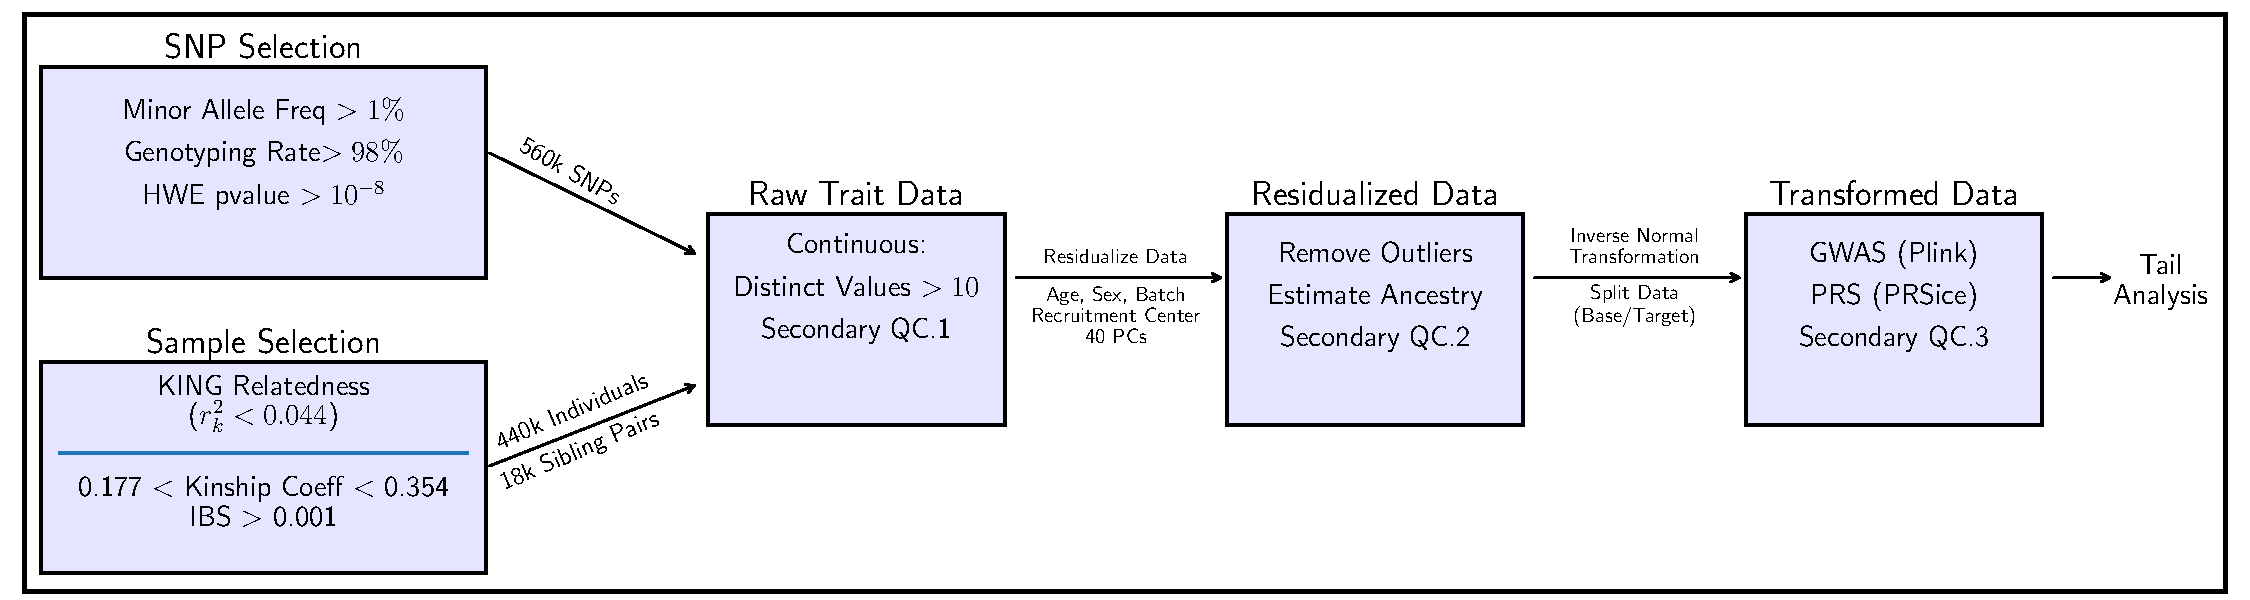
\includegraphics[trim=0cm 0cm 0cm 0cm, clip, width=\linewidth]{Figures/methodFlow.pdf} \end{maybe}
%\caption{\footnotesize{\textbf{Sample and SNP Workflow}}} \label{fig:qcFlow} \end{figure} \FloatBarrier



%\begin{figure}[!ht] \centering \begin{maybe}{showFig} 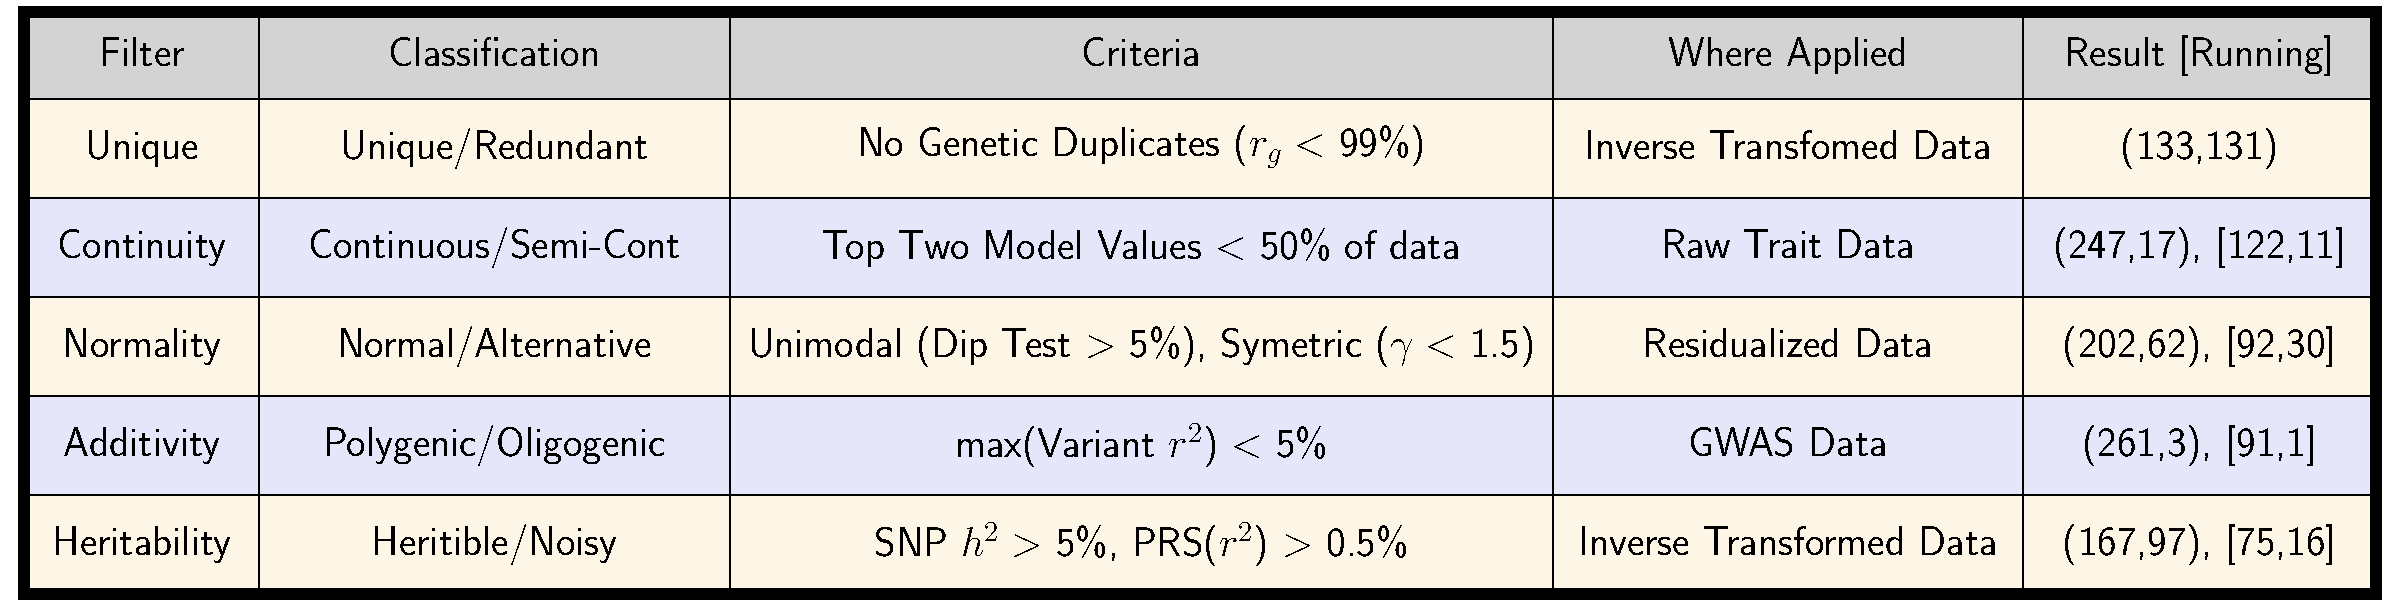
\includegraphics[trim=0cm 0cm 0cm 0cm, clip, width=16.5cm]{Figures/qctable.pdf} \end{maybe} \label{fig:m2} \caption{\scriptsize Secondary QC} \end{figure} 
%\clearpage \newpage

%\section*{Addendum 3: Lifetime Reproductive Success} \label{sec:supplement}

%\FloatBarrier \begin{figure}[!h] \centering \begin{maybe}{showFig} 
\includegraphics[trim=0cm 0cm 0cm 0cm, clip, width=16.5cm]{Figures/vishtable.pdf} \end{maybe} 
%\caption{\footnotesize{\textbf{Comparison of Selection Estimates}}} \label{fig:vishy} \end{figure} \FloatBarrier 

%\clearpage \newpage
%
%
%
%
%
%
\clearpage \newpage
\end{document}
